% ---------------------------------------------------------------------------------------------------------------
% TEMPLATE PARA TRABALHO DE CONCLUSÃO DE CURSO
% Universidade Federal do Pará
% Modelo da Faculdade de Engenharia Mecânica
% Idealizado por Sérgio Custódio e Kelvin Pinheiro
% Baseado no projeto: http://tcc.tsi.gp.utfpr.edu.br/paginas/modelos-latex-da-utfpr
% De:         Diego Marczal e 
% 	          Michael Vornes 
% ---------------------------------------------------------------------------------------------------------------

% CARREGA CLASSE PERSONALIZADA DA FEM/UFPA--------------------------------------------------------------------------
\documentclass[%twoside,                   % Impressão em frente e verso
oneside,                                   % Impressão apenas frente
]{ufpa-fem-abntex2}

%INCLUI ARQUIVOS DO TRABALHO DE CONCLUSÃO DE CURSO (PRÉ-TEXTUAIS, TEXTUAIS, PÓS-TEXTUAIS)-----------------------
%%%%%

% INSERE CAPA E FOLHA DE ROSTO
% CAPA-------------------------------------------------------------------

% ORIENTAÇÕES GERAIS-------------------------------------------------------------------------------------
% Caso algum dos campos não se aplique ao seu trabalho, como por exemplo,
% se não houve coorientador, apenas deixe vazio.
% Exemplos: 
% \coorientador{}
% \departamento{}

% DADOS DO TRABALHO--------------------------------------------------------------------------------------
\titulo{\textbf{CONTROLE DO MOVIMENTO DE CÂMERA COM BASE EM SENSORES DE POSIÇÃO DE UM SMARTFONE}}
\subtitulo{} %Se não hover subtítulo, deixar em branco.
\titleabstract{CAMERA MOTION CONTROL BASED ON MOBILE PHONE SENSORS DATA}
\autor{RAFFAELLO SALVETTI SANTOS}
\autorcitacao{SALVETTI, Raffaello} % Sobrenome em maiúsculo
\local{SALVADOR/BA}
\data{2019}

% NATUREZA DO TRABALHO-----------------------------------------------------------------------------------
\projeto{Trabalho de Conclusão de Curso}

% TÍTULO ACADÊMICO---------------------------------------------------------------------------------------
\tituloAcademico{Bacharel}

% ÁREA DE CONCENTRAÇÃO E LINHA DE PESQUISA---------------------------------------------------------------
% Se a natureza for Trabalho de Conclusão de Curso, deixe ambos os campos vazios
% Se for programa de Pós-graduação, indique a área de concentração e a linha de pesquisa
\areaconcentracao{}
\linhapesquisa{}

% DADOS DA INSTITUIÇÃO-----------------------------------------------------------------------------------
% Se a natureza for Trabalho de Conclusão de Curso, coloque o nome do curso de graduação em "programa"
% Formato para o logo da Instituição: \logoinstituicao{<escala>}{<caminho/nome do arquivo>}
\instituicao{Universidade Federal da Bahia}
\departamento{Escola Politécnica}
\programa{Curso de Graduação em Engenharia de Computação}
\logoinstituicao{2cm}{figuras/naomexafig/logoufba.png} %

% DADOS DOS ORIENTADORES---------------------------------------------------------------------------------
\orientador{Prof. Paulo César Machado de Abreu Farias}
%\orientador[Orientadora:]{Nome da orientadora}
\instOrientador{Universidade Federal da Bahia}

%\coorientador{Nome do coorientador}
%\coorientador[Coorientadora:]{Nome da coorientadora}
%\instCoorientador{Instituição do coorientador}

% FOLHA DE ROSTO-------------------------------------------------------------------

% Este arquivo não precisa ser alterado

%% TRABALHO DE CONCLUSÃO DE CURSO
\preambulo{{\imprimirprojeto}, apresentado como parte dos requisitos para a obtenção de grau de {\imprimirtituloAcademico} em Engenharia de Computação, pela {\imprimirinstituicao}.}

% ---
% Inserir folha de aprovação
% ---
% Isto é um exemplo de Folha de aprovação, elemento obrigatório da NBR
% 14724/2011 (seção 4.2.1.3). Você pode utilizar este modelo até a aprovação do trabalho. Após isso, substitua todo o conteúdo deste arquivo por uma imagem da página assinada pela banca com o comando abaixo:
%
% \includepdf{folhadeaprovacao_final.pdf}
%


%\dataaprovacao{00/00/0000}
%\conceito{} %Antes da defesa, não adicionar valor ao compo. Após a defesa, pode-se adicionar Regular, Bom ou Excelente e solicitar as assinaturas da banca examinadora.
 
\nomePrimeiromembro{Prof. Jés de Jesus Fiais Cerqueira}
\instPrimeiromembro{UFBA}
 
\nomeSegundomembro{Prof. Tiago Trindade Ribeiro}
\instSegundomembro{UFBA}

%Ocultar ou não dependendo do número de professores na banca. Ver arquivo de configuracao \assinatura{\imprimirnomeTerceiromembro  \\ Membro - \imprimirinstTerceiromembro}  nas configuracoes ufpa-fem-abntex2.cls.

%\nomeTerceiromembro{Eng. Beltrano Cunha} 
%\instTerceiromembro{Externo (PETROBRAS)}

%ª
 


\begin{document}
	\pretextual
	\imprimircapa                                  \imprimirfolhaderosto{}                           
	\imprimirfolhadeaprovacao{} 
	% DEDICATÓRIA------------------------------------------------------------------

\renewcommand{\dedicatorianame}{DEDICATÓRIA}

\begin{dedicatoria}

Dedico à família e aos amigos.

\end{dedicatoria}

	% AGRADECIMENTOS---------------------------------------------------------------

\begin{agradecimentos}[AGRADECIMENTOS]

Agradeço à Deus por permitir que eu chegasse até aqui. À minha família, em especial à minha mãe Sonia e ao meu pai Rui, que se esforçaram para me proporcionar conforto e educação. À minha irmã Alessandra, meus avós Lori e Luigi, às minhas tias Silvana e Zete, que incentivaram minha criatividade desde criança. À Mariana, minha companheira que sempre esteve ao meu lado, com bastante paciência, me apoiando e ajudando a vencer batalhas. Aos meus sogros Eugênio e Luiza, e cunhado Francisco que me acolheram e torceram muito por mim durante essa jornada. Aos meus amigos que estiveram junto também nas horas de dificuldade. Agradeço ao professor Heraldo, que muito contribuiu para minha formação intelectual e me apontou o caminho ainda no ensino médio. Ao meu orientador Paulo César, pelo suporte necessário para a realização deste trabalho. À Universidade Federal da Bahia e sua equipe de excelentes professores, com os quais tive a oportunidade de aprender. Por fim, agradeço aos meus colegas de curso, principalmente à Felipe, Luciano e Hugo, que tornaram essa caminhada mais descontraída.

\end{agradecimentos}

	% EPÍGRAFE---------------------------------------------------------------------

\renewcommand{\epigraphname}{EPÍGRAFE}

\begin{epigrafe}

\textit{"Se o conhecimento traz problemas, não é a ignorância que os resolve." (Isaac Asimov)}

\end{epigrafe}

% OBSERVAÇÕES------------------------------------------------------------------
% Altere o texto para inserir a epígrafe do seu trabalho


	% RESUMO--------------------------------------------------------------------------------

\begin{resumo}[RESUMO]
\begin{SingleSpacing}

Sistemas robóticos fazem parte da história humana. Seja na vida pratica, nos dias atuais, ou nas fantasias criadas por cineastas e escritores, bem antes da computação ser criada.\\

\textbf{Palavras-chave}: Robótica, Movimento, Controle, Automação, Câmera.

\end{SingleSpacing}
\end{resumo}

% OBSERVAÇÕES---------------------------------------------------------------------------
% Altere o texto inserindo o Resumo do seu trabalho.
% Escolha de 3 a 5 palavras ou termos que descrevam bem o seu trabalho .
% As palavras-chave são separadas por pontos. Apenas a primeira letra é maiúscula.

 % Resumo em Português
	% ABSTRACT--------------------------------------------------------------------------------

\begin{resumo}[ABSTRACT]
\begin{SingleSpacing}


Write your abstract here!!!\\

\textbf{Keywords}: Keywords 1. Keywords 2. Keywords 3. Keywords 4.

\end{SingleSpacing}
\end{resumo}

% OBSERVAÇÕES---------------------------------------------------------------------------
% Altere o texto inserindo o Abstract do seu trabalho.
% Escolha de 3 a 5 palavras ou termos que descrevam bem o seu trabalho 
% As palavras-chave são separadas por pontos. Apenas a primeira letra é maiúscula. % Resumo em Inglês
	% Lista de Figuras----------------------------------------------------------------

\pdfbookmark[0]{\listfigurename}{lof}
\listoffigures*
\cleardoublepage

% OBSERVAÇÕES---------------------------------------------------------------------
% Este arquivo não precisa de ser alterado, pois a lista é gerada automaticamente.

	%% LISTA DE QUADROS----------------------------------------------------------------

\renewcommand{\listofquadrosname}{LISTA DE QUADROS}

\pdfbookmark[0]{\listofquadrosname}{loq}
\listofquadros*
\cleardoublepage

% OBSERVAÇÕES---------------------------------------------------------------------
% Este arquivo não necessita de ser editado. A lista é gerada automaticamente.

	% LISTA DE TABELAS-------------------------------------------------------------

\pdfbookmark[0]{\listtablename}{lot}
\listoftables*
\cleardoublepage

% OBSERVAÇÕES-------------------------------------------------------------------
% Este arquivo não precisa ser alterado, pois a lista é gerada automaticamente.
 % Lista de Tabelas
	% LISTA DE ABREVIATURAS E SIGLAS----------------------------------------------------------

\begin{siglas}
	\item[API]         Application Programming Interface
	\item[ARM]         Advanced RISC Machine
	\item[ATX]         Advanced Technology eXtended
	\item[DOF]         Degrees of freedom
	\item[GPIO]        General-Purpose Input/Output
	\item[HAL]         Hardware Abstraction Layer
	\item[IP]          Internet Protocol
	\item[MCC]         Módulo de Controle de Câmera
	\item[MCM]         Módulo de Captura de Movimento
	\item[PAN]         Panning
	\item[PSU]         Power Supply Unit
	\item[PWM]         Pulse-Width Modulation
	\item[RAM]         Random Access memory
	\item[ROS]		   Robot Operating System
	\item[RTP]         Real Time Protocol
	\item[SoC]         System on Chip
	\item[TCP]         Transmission Control Protocol
	\item[TILT]        Tilting
	\item[VLC]         VideoLAN Client
	\item[VR]          Virtual Reality
\end{siglas}

% OBSERVAÇÕES-----------------------------------------------------------------------------
% Altere a lista acima para definir os acrônimos e siglas utilizados neste trabalho

	% LISTA DE SÍMBOLOS------------------------------------------------------------

\begin{simbolos}
    \item[$ \theta $] Ângulo de Rotação
    \item[$ \Delta_x $] Compoenente $x$ do Vetor de Rotação
    \item[$ \Delta_y $] Compoenente $y$ do Vetor de Rotação
    \item[$ \Delta_z $] Compoenente $z$ do Vetor de Rotação
\end{simbolos}

% OBSERVAÇÕES-------------------------------------------------------------------
% Altere a lista acima para definir os símbolos utilizados no trabalho

	%% LISTA DE ALGORITMOS----------------------------------------------------------

\newcommand{\algoritmoname}{Algoritmo}
\renewcommand{\listalgorithmcfname}{LISTA DE ALGORITMOS}

\floatname{algocf}{\algoritmoname}
\newlistof{listofalgoritmos}{loa}{\listalgoritmoname}
\newlistentry{algocf}{loa}{0}

\counterwithout{algocf}{chapter}
\renewcommand{\cftalgocfname}{\algoritmoname\space}
\renewcommand*{\cftalgocfaftersnum}{\hfill--\hfill}

\pdfbookmark[0]{\listalgorithmcfname}{loa}
\listofalgorithms
\cleardoublepage

% OBSERVAÇÕES------------------------------------------------------------------
% Este arquivo não precisa ser alterado, pois a lista é gerada automaticamente.

	% SUMÁRIO----------------------------------------------------------------------

\renewcommand{\contentsname}{SUMÁRIO}

\pdfbookmark[0]{\contentsname}{toc}
\tableofcontents*
\cleardoublepage

% OBSERVAÇÕES-------------------------------------------------------------------
% Este arquivo não precisa ser alterado, pois o sumário é gerado automaticamente.

	%Verificar folha de Aprovação e Catalogação Bibliográfica
	
	% Sumário
	
	\textual
	\begin{OnehalfSpace}
	% INSERE ELEMENTOS TEXTUAIS
	% INTRODUÇÃO-------------------------------------------------------------------

\chapter{INTRODUÇÃO}
\label{chap:introducao}

Dutos de ventilação usados nos sistemas de ar-condicionado estão sujeitos a diversos tipos de danos, dentre os quais pode-se listar os entupimentos progressivos devido ao acúmulo de poeira e de pequenos animais mortos. \citeonline{carmo1999qualidade} Por normalmente ser locais de difícil acesso, apresentam dificuldades em sua manutenção, favorecendo a proliferação de bactérias e transmissão de vírus \citeonline{bortoletto2002contaminaccao}.\par
Subestações de energia elétrica, em grande parte das vezes, ficam expostas a intempéries, que causam oxidações em suportes, equipamentos e cabos. Sua inspeção oferece riscos a vida por expor o corpo humano a uma quantidade enorme de energia. Apesar de existir uma norma rigorosa para a realização de inspeções preventivas, acidentes com vítima ainda acontecem \citeonline{santos2012inspeccao}.\par
A inspeção de reservatórios de produtos químicos requer uma minuciosa análise estrutural, uma busca por áreas oxidadas e falhas em pontos de solda, tarefa que demanda muitas horas de trabalho humano. A exposição a gases e vapores tóxicos, por menor que seja a quantidade, causam riscos à saúde do inspetor \citeonline{molina2008metodo}.\par
Os casos citados, são apenas algumas das atividades extremamente necessárias no ambiente industrial, que expõem a saúde das pessoas a riscos que poderiam ser evitados, através do uso de dispositivos especializados. \par 
Robôs equipados com ferramentas adequadas para cada tarefa, dotados de um sistema de navegação autônomo ou por controle remoto, podem ser usados para evitar ou minimizar os riscos à saúde dos inspetores. Como exemplo, o robô \textit{SENSABOT}, usado pela Shell, para monitorar e inspecionar plantas de óleo e gás, mostrado na \autoref{fig:sensabot}, e o robô \textit{ABB}, usado em inspeções de transformadores, sem a necessidade de drenar o óleo, visto na \autoref{fig:abb}. Contudo o uso de robôs não se restringe apenas ao ambiente industrial. No ano de 2011, robôs submarinos foram protagonistas na localização e resgate das peças do avião da Air France 447, que caiu no Oceano Atlântico em 2009. Foram usados robôs de inspeção, para verificar as condições estruturais da usina nuclear de Fukushima Daiichi no Japão, que foi afetada por um tsunami. 

\begin{figure}[H]
	\centering
	\begin{subfigure}{.5\textwidth}
		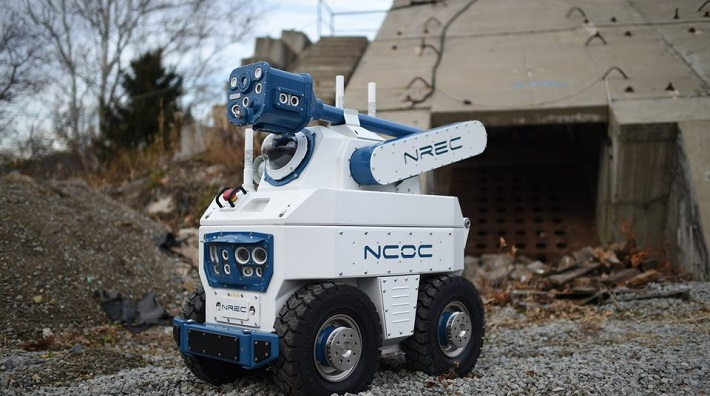
\includegraphics[width=0.95\textwidth]{figuras/sensabot.jpg}
		\caption{SENSABOT}
		\fonte{\citeonline{tractica2019sensabot}.}
		\label{fig:sensabot}
	\end{subfigure}%
	\begin{subfigure}{.5\textwidth}
		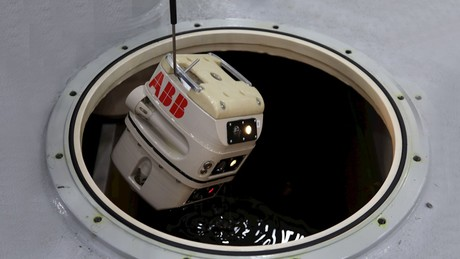
\includegraphics[width=0.95\textwidth]{figuras/abb.jpg}
		\caption{ABB}
		\fonte{\citeonline{processonline2019abb}.}
		\label{fig:abb}
	\end{subfigure}
	\caption{Robôs de inspeção}
\end{figure}

Independente de um robô ser controlado diretamente por uma pessoa, ou operar em modo completamente autônomo, em algum momento, a observação, supervisão e o julgamento humano ainda é um elemento crítico da atividade robótica.\par

A maior ligação perceptiva entre um ambiente remoto e o operador de um robô, acontece através do vídeo enviado por uma (ou mais) câmera montada no robô. Existe uma relação forte entre problemas de localização da câmera e sua montagem, bem como ângulo de visão e outros fatores que podem degradar essa ligação e deixar o operador vulnerável a uma série de erros tais como: desorientação, falha ao reconhecer danos ou simplesmente não notar um ponto importante durante uma inspeção.\par

Estudos sugerem que disponibilizar uma câmera controlada independentemente da orientação de um robô, pode facilitar tarefas de localização num ambiente. \citeonline{hughes2004robotic}

A complexidade de operação de um robô é proporcional ao seu DOF (\textit{Degrees of Freedom}), isto é, quanto maior a variedade de movimentos o robô pode executar (considerando seu deslocamento, movimento de braços mecânicos e câmera), mais difícil é o controle manual para o operador.
Pensando nisso, o desenvolvimento de controles mais intuitivos para a câmera embarcada diminui a complexidade geral do controle de movimentos globais do robô. \par

Com o objetivo de aprofundar os conhecimentos adquiridos ao longo do curso, este trabalho visa criar um controle de câmera do tipo \textit{Pan} e \textit{Tilt}, baseando-se nos dados de movimento, coletados e enviados, através de rede sem fio, por um \textit{smartphone} acoplado à cabeça do operador, por um óculos VR (\textit{Virtual Reality}). Dessa forma, os movimentos de rotação da cabeça do operador (\textit{yaw} e \textit{pitch}) são traduzidos em movimentos da câmera (\textit{Pan} e \textit{Tilt}), montada no robô. \par 

No projeto, pretende-se utilizar um \textit{Raspberry Pi}, como unidade computacional e de controle dos servo motores da câmera, e um celular \textit{smartphone} \textit{Android}, responsável por coletar e enviar informações referentes a posição espacial do aparelho. \par

Com o desenvolvimento do projeto, procura-se um melhor entendimento em aspectos relacionados a rede de computadores, sistemas operacionais, interfaces de hardware, modulação por largura de pulso, eletrônica geral e desenvolvimento de sistemas para plataformas móveis.\par

Competências ligadas a construção de software, utilizando múltiplas linguagens de programação, devem ser evoluídas, já que o módulo de controle, embarcado no \textit{Raspberry Pi}, deve ser construído em linguagem C e o módulo de coleta de dados desenvolvido em Java, usando a API (\textit{Application Programming Interface}) fornecida pelo sistema operacional \textit{Android}.\par


	%% REVISÃO DE LITERATURA--------------------------------------------------------

\chapter{REVISÃO BIBLIOGRÁFICA}
\label{chap:fundamentacaoTeorica}

\section{Turbinas hidrocinéticas}

A potencia gerada por uma turbina pode ser expressa pela \autoref{eq:Power}.

\begin{equation}
P = \frac{1}{2}A\rho {V^3}{C_P}
\label{eq:Power}
\end{equation}

Sendo $A$ a área do rotor da turbina ($m^2$), $\rho$ a massa específica do fluido ($kg/{m}^3$), $V$ é a velocidade de corrente ($m/s$) e $C_P$ o coeficiente de potência (adimensional). O coeficiente de potência de uma turbina hidrocinética indica a quantidade de energia mecânica extraída a partir da energia disponível no fluido. A máxima eficiência que uma turbina hidrocinética ideal pode alcançar é dada pelo Limite de Betz-Joukowski que corresponde a 59,3\%, o equivalente a um $C_P$ de 0,593 \cite{vallverdu2014, SHINOMIYA2015d}.

\subsection{Princípios de funcionamento, classificação e principais componentes}

A \autoref{fig:Behrouzi2014-2} apresenta algumas configurações possíveis.

\begin{figure}
	\centering
	\begin{subfigure}{0.31\textwidth}
		\centering
		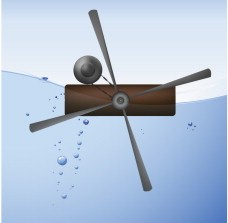
\includegraphics[scale=0.9]{figuras/VermaakVa.jpg}
		\caption{Eixo no plano.}
		\label{subfig:Inplane}
	\end{subfigure}
	\begin{subfigure}{0.31\textwidth}
		\centering
		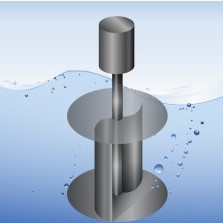
\includegraphics[scale=0.9]{figuras/VermaakVf.jpg}
		\caption{Savonius.}
		\label{subfig:Savonius}
	\end{subfigure}
	\begin{subfigure}{0.31\textwidth}
		\centering
		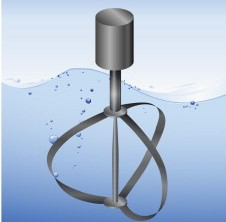
\includegraphics[scale=0.9]{figuras/VermaakVd.jpg}
		\caption{Darrieus.}
		\label{subfig:Darrieus}
	\end{subfigure}
	\begin{subfigure}{0.31\textwidth}
		\centering
		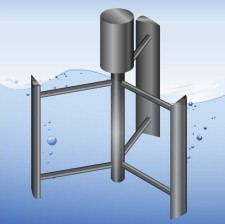
\includegraphics[scale=0.9]{figuras/VermaakVc.jpg}
		\caption{Darrieus - H.}
		\label{subfig:DarrieusH}
	\end{subfigure}	
	\begin{subfigure}{0.31\textwidth}
		\centering
		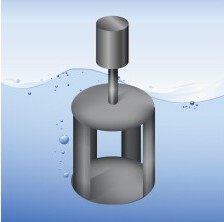
\includegraphics[scale=0.9]{figuras/VermaakVb.jpg}
		\caption{Darrieus gaiola de esquilo.}
		\label{subfig:SquirrelcageDarrieus}
	\end{subfigure}
	\begin{subfigure}{0.31\textwidth}
		\centering
		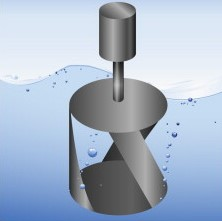
\includegraphics[scale=0.9]{figuras/VermaakVe.jpg}
		\caption{Gorlov.}
		\label{subfig:Gorlov}
	\end{subfigure}	
	\caption{Turbinas hidrocinéticas de eixo vertical.}
	\fonte{\citeonline{harris2006essential}.}
	\label{fig:Behrouzi2014-2}
\end{figure}

\subsection{Modelos de predição de performance hidrodinâmica}

Uma revisão sobre modelos de predição de performance para turbinas eólicas de eixo vertical incluem os trabalhos de \citeonline{Brahimi1995}, \citeonline{paraschivoiu2002prediction}, \citeonline{paraschivoiu2002wind} e \citeonline{ISLAM20081087},  que serviram como ponto de partida para os modelos hidrodinâmicos \cite{Dai2011}. 

	% FUNDAMENTAÇÃO TEÓRICA--------------------------------------------------------

\chapter{FUNDAMENTAÇÃO TEÓRICA}
\label{chap:fundamentacao-teorica}

Este capítulo descreve as tecnologias e conceitos centrais utilizados durante a
concepção do projeto. As definições apresentadas são embasadas no material bibliográfico
revisado, que serviu de apoio no desenvolvimento de um trabalho fundamentado nas teorias
existentes.

\section{Raspberry Pi}
\label{sec:raspi}

O Raspberry Pi é uma família de computadores em placa única (SOC em inglês), com o tamanho de um cartão de crédito. Inicialmente seu objetivo era promover o ensino de computação (programação) básica em escolas, principalmente públicas, de todo o mundo. Entretanto, por possuir poder computacional razoável, uma boa quantidade de memória ram (a partir do modelo B) e um preço relativamente baixo, passou a ser usado para outros objetivos como: console de videogame clássico (emulação de jogos), gerencia de mídia (vídeos, fotos e musicas), estudos em eletrônica, domótica (automação residencial), internet das coisas e robótica. \citeonline{jucapereira2018aplicacoes} \par
Uma versão do sistema operacional Debian Linux, chamada Raspbian, foi criada para o Raspberry Pi, portando também uma serie de aplicativos e ferramentas de desenvolvimentos já existentes para computadores da plataforma PC. Dessa modo, o desenvolvimento de programas se torna uma tarefa extremamente simples, já que o hardware é abstraído pelo sistema operacional, e não é necessário conhecimento especifico do hardware do Raspberry Pi (plataforma ARM). As linguagens mais utilizadas para desenvolvimento de software com bibliotecas disponíveis para interação com o hardware são o C/C++ e Python, porém, é possível desenvolver em outras linguagens de programação como o PHP e Java. \citeonline{jucapereira2018aplicacoes} \par

\begin{figure}[H]
	\centering
	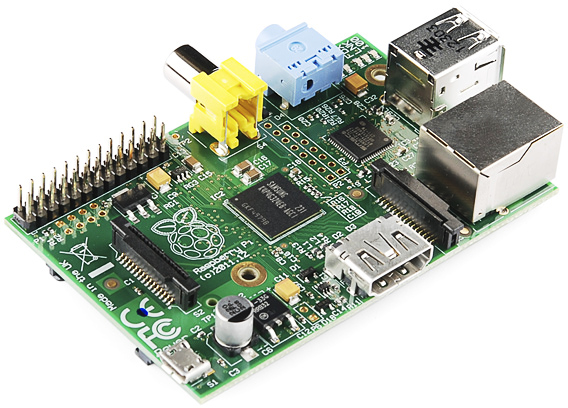
\includegraphics[width=0.6\textwidth]{figuras/raspberrypi_model_b.jpg}
	\caption{Raspberry Pi (Modelo B).}
	\fonte{ \citeonline{sparkfun2019}}
	\label{fig:raspi_modelb}
\end{figure}

\section{Servo Motor}
\label{sec:servomotor}

Um servo motor, visto na \autoref{fig:servo_g9}, é um atuador rotatório, ou atuador linear, que permite um controle preciso da posição linear ou angular, velocidade e aceleração de uma carga ligada ao seu eixo. Consiste basicamente em um motor de corrente continua (para o caso particular desse trabalho), acoplado a um sensor (potenciômetro), como ilustrado na \autoref{fig:insideaservo}, para ler sua posição durante o movimento. Normalmente, os motores servos necessitam de um sinal de controle modulado por largura de pulso (PWM em ingles) para operar. \citeonline{petruzella2009electric} \par

\begin{figure}[h]
	\centering
	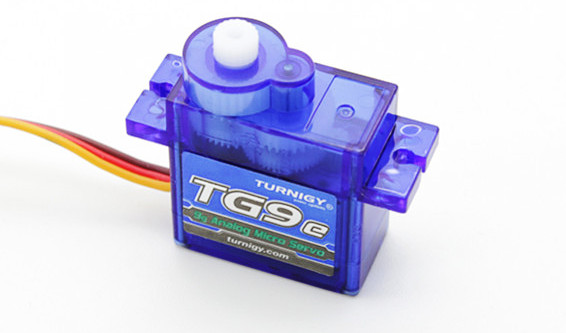
\includegraphics[width=0.6\textwidth]{figuras/servo_g9.jpg}
	\caption{Servo Micro TG9.}
	\fonte{ \citeonline{hobbyking2019}}
	\label{fig:servo_g9}
\end{figure}

O servo motor opera em malha fechada, isto é, seu controlador compara a velocidade de movimento e sua posição para gerar o próximo comando de movimento, minimizando o erro. \citeonline{petruzella2009electric} O esquema de funcionamento do servo motor é mostrado na figura \autoref{fig:servo_closed_loop}. 

\begin{figure}[h]
	\centering
	\begin{subfigure}{.5\textwidth}
		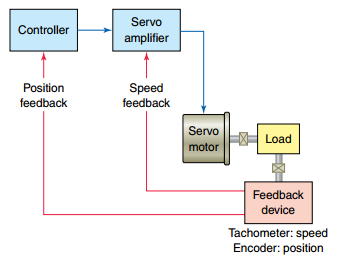
\includegraphics[width=0.95\textwidth]{figuras/servo_closed_loop.png}
		\caption{Sistema em malha fechada.}
		\fonte{ \citeonline{petruzella2009electric}}
		\label{fig:servo_closed_loop}
	\end{subfigure}%
	\begin{subfigure}{.5\textwidth}
		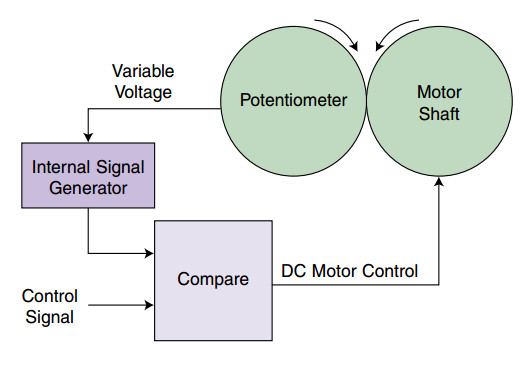
\includegraphics[width=0.95\textwidth]{figuras/inside_a_servo.jpg}
		\caption{Componentes internos.}
		\fonte{\citeonline{pinckney2006pulse}.}
		\label{fig:insideaservo}
	\end{subfigure}
	\caption{Sistema de controle de um servo motor.}
\end{figure}

\section{Modulação por Largura de Pulso}
\label{sec:pwm}

A modulação por largura de pulso é uma técnica empregada em diversas áreas da eletrônica, sendo utilizada para controlar fontes chaveadas, velocidade de motores, luminosidade, servo motores e diversas outras aplicações. Consiste em variar a o tempo em que um pulso de tensão oscila entre os níveis alto e baixo numa taxa rápida o suficiente para que a média dos pulsos crie um valor médio de tensão efetivo, ilustrado na \autoref{fig:pwm}. Ao valor definido pela divisão entre: a largura de pulso com a tensão em nível alto, e o período do sinal; é dado o nome ciclo de trabalho ou \textit{dutty cycle}. Variar o \textit{dutty cycle} significa variar a tensão média, isto é, a potência é proporcional a tensão média resultante. \citeonline{pinckney2006pulse}.

\begin{figure}[h]
	\centering
	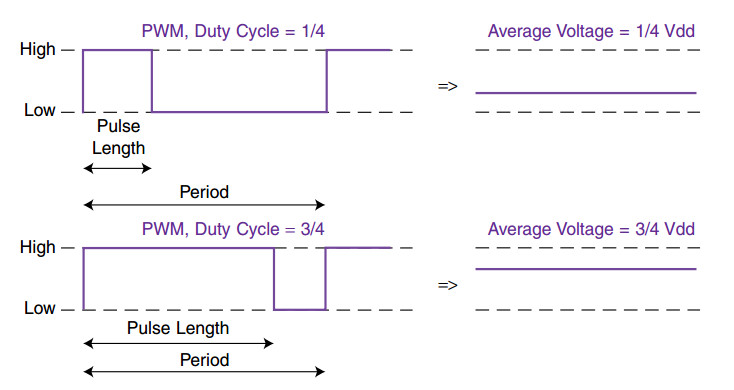
\includegraphics[width=1\textwidth]{figuras/pwm.jpg}
	\caption{Modulação por largura de pulso e tensão média resultante}
	\fonte{ \citeonline{pinckney2006pulse}}
	\label{fig:pwm}
\end{figure}

A largura de pulso pode ser calculada usando a equação \autoref{eq:duttycicle}.

\begin{equation}
{Dutty Cycle} = 100 \times \frac{Largura do Pulso}{Período}  
\label{eq:duttycicle}
\end{equation}

Onde: Duty Cycle é um valor dado em porcento, Largura do pulso e Período são valores dados em segundos.\par

Uma vez calculado o ciclo de trabalho, é possível calcular o valor da tensão média gerada pelo sinal através da \autoref{eq:avervoltage}.

\begin{equation}
{Tensão Média} = {Tensão do Pulso} \times {Duty Cycle}
\label{eq:avervoltage}
\end{equation}

\section{Smartfone Android}
\label{sec:android}

O smartfone é um dispositivo móvel que mescla recursos de um telefone celular (receber e efetuar chamadas, mensagens de texto curto e etc) e recursos de um computador pessoal garantindo a possibilidade de instalar novos aplicativos e assim, agregar novas funcionalidades ao aparelho.\par

O Android é um sistema operacional de código livre, baseado em núcleo Linux (responsável por gerenciar dispositivos de entrada e saída, memória e processos), marcado em vermelho na \autoref{fig:androidsysarch}, e desenvolvido por uma das maiores empresas de tecnologia da atualidade, a Google. \citeonline{ronamadeo2018} Sua interface com o usuário é baseada na manipulação direta, isto é, apresenta continuamente o objeto de interesse permitindo sua manipulação usando recursos que correspondem proximamente ao mundo físico. \citeonline{barbosa2010interaccao} Atualmente o sistema operacional Android pode ser encontrado em outros aparelhos como relógios, televisores e dispositivos gerenciadores de mídia. \citeonline{androidcom2019} \par

\begin{figure}[H]
	\centering
%	\begin{subfigure}{.5\textwidth}
		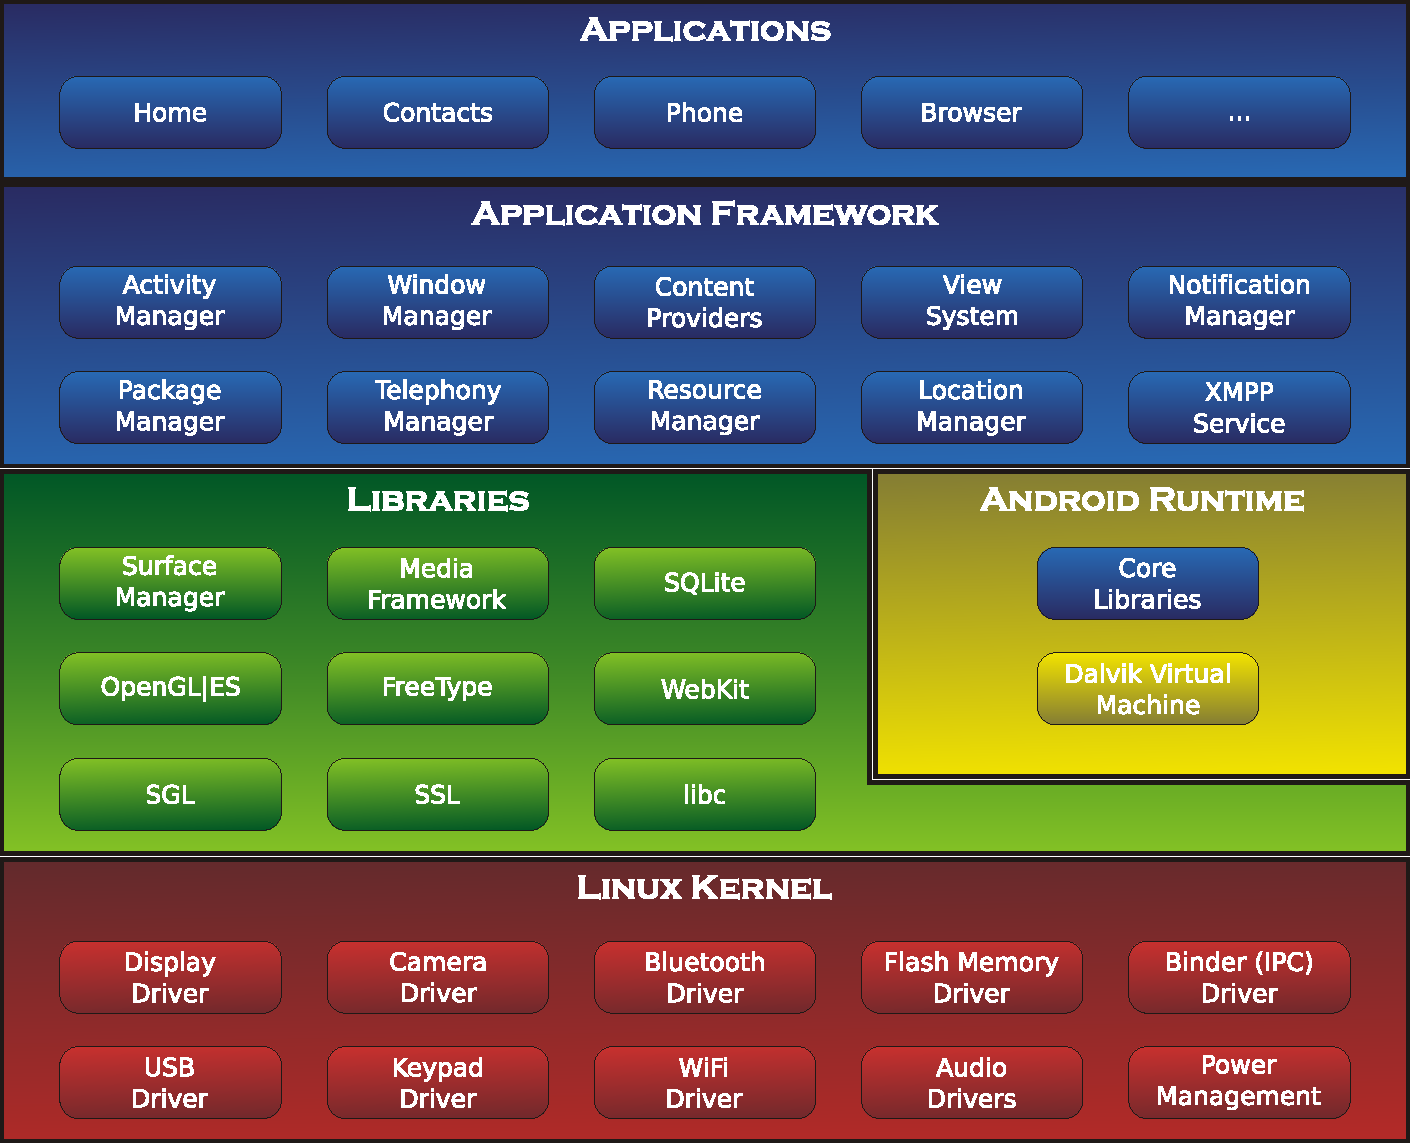
\includegraphics[width=0.7\textwidth]{figuras/android_sys_arch.pdf}
		\caption{Arquitetura do sistema operacional Android.}
		\fonte{ \citeonline{brady2008anatomy}.}
		\label{fig:androidsysarch}
%	\end{subfigure}%
%	\begin{subfigure}{.5\textwidth}
%		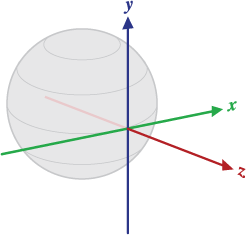
\includegraphics[width=0.95\textwidth]{figuras/axis_globe.png}
%		\caption{em relação ao globo terrestre.}
%		\label{fig:axisglobe}
%	\end{subfigure}
%	\caption{Sistema operacional Android.}
\end{figure}

Boa parte dos smartfones vendidos atualmente com o sistema operacional Android, possuem uma gama de sensores embutidos capazes de fornecer dados, com um grau de precisão aceitável, relativos a orientação e movimento do aparelho e até condições do ambiente como iluminação, pressão atmosférica e umidade do ar. \citeonline{androidcom2019} Esses sensores encontram-se divididos em três grupos básicos na API de desenvolvimento fornecida pelo Android. Sensores \textit{Ambientais}, que podem ser utilizados em aplicações simples como coletar o nível de iluminação do ambiente, a umidade e temperatura para calcular o ponto de orvalho (condição em que a água em vapor presente num ambiente se condensa tornando-se o orvalho), e os sensores de \textit{Posição} e \textit{Movimento}, que podem ser usados em aplicações como jogos que, por exemplo, utilizam a aceleração da gravidade para inferir movimentos complexos do usuário como rotações, sacudidas e inclinações do aparelho. Este último grupo sendo o ponto de interesse para o trabalho, e portanto detalhado adiante.\par

\subsection{Sensores de Movimento}
\label{subsec:motionsensors}

A plataforma de desenvolvimento do Android oferece vários sensores que permitem sentir o movimento de um dispositivo. Dentre eles, os mais utilizados são os sensores de gravidade, aceleração linear e vetor de rotação, que podem ser implementados em hardware ou software (baseando-se em dados fornecidos por outros sensores implementados em hardware), e os sensores acelerômetro e giroscópio, que sempre são implementados em hardware. Todos eles descrevem o movimento do dispositivo em formato matricial.\par

De forma geral, os sensores usam um sistema de coordenadas com três eixos para expressas os dados. Para a maioria dos sensores da API, o sistema de coordenadas é definido relativo a tela do dispositivo, quando segurado na orientação padrão (porta retrato para celulares e paisagem para tablets), como mostrado na \autoref{fig:axisdevice}. Dessa forma, o eixo X é horizontal e aponta para a direita, o eixo Y é vertical e aponta para cima e o eixo Z, perpendicular a tela do dispositivo, estando seus valores positivos do lado da tela e os negativos atrás da tela. Um ponto importante de ser notado, é que a orientação do sistema de eixos não muda quando o dispositivo é segurado de maneira diferente da sua orientação padrão.\par

\begin{figure}[H]
	\centering
	\begin{subfigure}{.5\textwidth}
		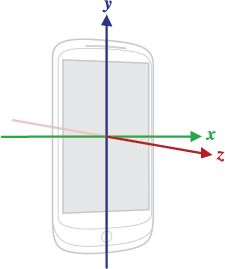
\includegraphics[width=0.85\textwidth]{figuras/axis_device.png}
		\caption{em relação ao aparelho.}
		\label{fig:axisdevice}
	\end{subfigure}%
	\begin{subfigure}{.5\textwidth}
		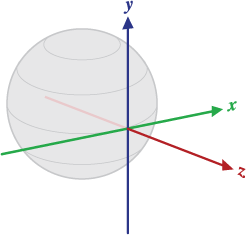
\includegraphics[width=0.95\textwidth]{figuras/axis_globe.png}
		\caption{em relação ao globo terrestre.}
		\label{fig:axisglobe}
	\end{subfigure}
	\caption{Sistema de coordenadas.}
	\fonte{ \citeonline{google2019devsensors}.}
\end{figure}

O sensor vetor de rotação representa a orientação do dispositivo como uma combinação  de um angulo e um eixo no qual o dispositivo rotacionou com um ângulo $\theta$ em torno de um eixo (x, y ou z). \citeonline{google2019devsensors} \par
Os três componentes do vetor re rotação são expressos como:\\

\begin{equation}
\Delta_x = x \times sen(\frac{\theta}{2})
\label{eq:vec_rot_x}
\end{equation}

\begin{equation}
\Delta_y = y \times sen(\frac{\theta}{2})
\label{eq:vec_rot_y}
\end{equation}

\begin{equation}
\Delta_z = z \times sen(\frac{\theta}{2})
\label{eq:vec_rot_z}
\end{equation}

Onde a magnitude do vetor de rotação é expresso por $sen(\frac{\theta}{2})$, e sua direção é a mesma do eixo de rotação.\par

A o sistema de coordenada de referencia é definido como uma base ortogonal direta, como mostrado na \autoref{fig:axisglobe}, e possui as seguintes características:\par
\begin{itemize}
\item O eixo X é definido como o produto vetorial dos eixos Y e Z, é tangente a superfície terrestre no local onde o dispositivo se encontra e aponta aproximadamente para o leste.\par

\item O eixo Y é tangente a superfície terrestre no local onde o dispositivo se encontra e aponta para o norte magnético. \par

\item O eixo Z aponta para o céu e é perpendicular ao solo.
\end{itemize}
	%% METODOLOGIA------------------------------------------------------------------

\chapter{METODOLOGIA}
\label{chap:metodologia}

Este trabalho ...

\section{Análise modal numérica}
\label{sec:metmodal}

A análise modal numérica...

\section{Double-multiple streamtube model}
\label{sec:metbet}

O código computacional responsável por fornecer os dados de forças e torque atuantes na turbina utiliza ...
 

	% METODOLOGIA------------------------------------------------------------------

\chapter{Implementação do Protótipo}
\label{chap:prototipo}

Este capítulo descreve a montagem do protótipo para testes. Será feita uma introdução do funcionamento geral, e suas principais características. Posteriormente, será mostrado o funcionamento da base de testes da câmera, conexões entre os servo motores e os pinos GPIOs (\textit{General-Purpose Input/Output}) do \textit{Raspberry Pi}, desenvolvimento do programa de controle dos servo motores, desenvolvimento do aplicativo \textit{Android}, responsável por capturar dados dos sensores de posição e enviá-los pela rede sem fio.

\section{Conceito}
\label{sec:conceito}

A ideia central do projeto é trazer ao operador de um robô de inspeção, um controle intuitivo para câmera embarcada. Pretende-se criar a sensação de imersividade, isto é, projetar o operador no ambiente inspecionado, através da visão \textit{stereo}, simulada no protótipo por apenas uma câmera, e a tradução dos movimentos da cabeça do operador em movimentos da câmera embarcada.\par
Para atingir este objetivo, um celular será acoplado à cabeça do operador, através de um óculos VR (Google \textit{cardboard}), ilustrado na \autoref{fig:googlecardboard}. Prende-se o óculos à cabeça por uma alça, fixada com \textit{Velcro}, indicado com as marcações verdes da \autoref{fig:googlecardboard_welcro}. \par 

\begin{figure}[H]
	\centering
	\begin{subfigure}{.5\textwidth}
		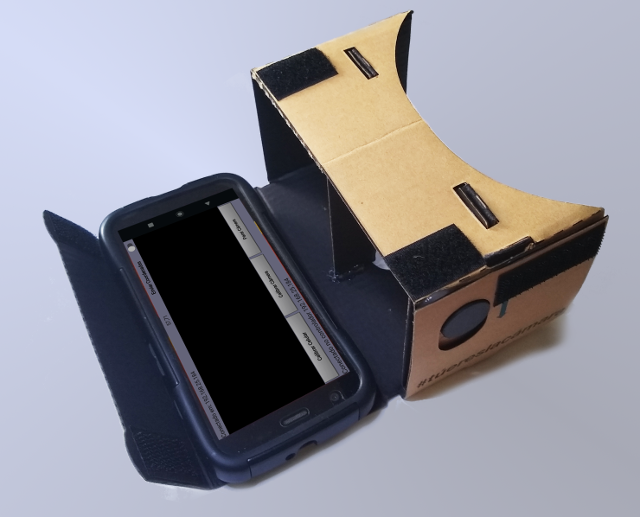
\includegraphics[width=0.95\textwidth]{figuras/cardboard1.png}
		\caption{visão fontal (compartimento do celular).}
	\end{subfigure}%
	\begin{subfigure}{.5\textwidth}
		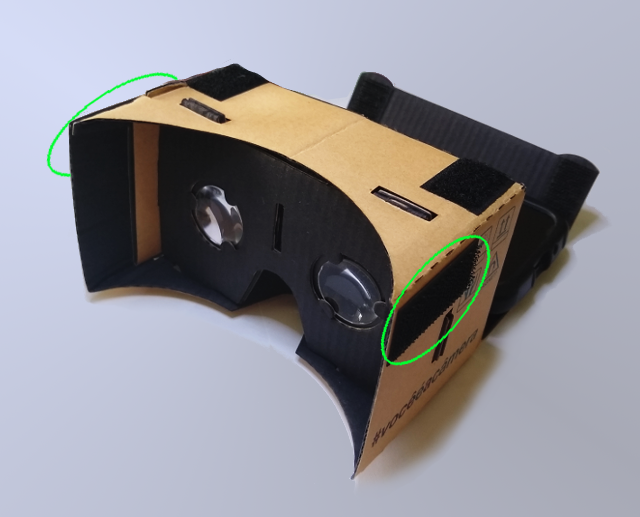
\includegraphics[width=0.95\textwidth]{figuras/cardboard2.png}
		\caption{visão traseira (lentes).}
		\label{fig:googlecardboard_welcro}
	\end{subfigure}
	\caption{Google Cardboard.}
	\label{fig:googlecardboard}
\end{figure}

Os sensores do celular capturam os movimentos rotacionais da cabeça do operador, como mostra a sequência da \autoref{fig:headmotion}, e enviam os sinais capturados para o centro de controle, um \textit{Raspberry Pi} embarcado junto com uma câmera e seus atuadores.\par

\begin{figure}[H]
	\centering
	\begin{subfigure}{.5\textwidth}
		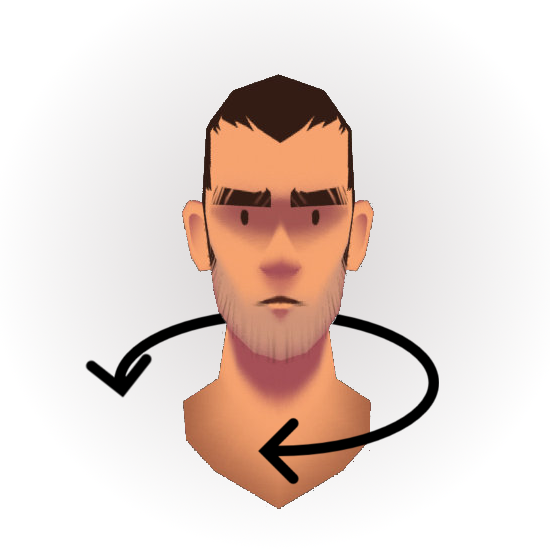
\includegraphics[width=0.95\textwidth]{figuras/yaw.png}
		\caption{rotação horizontal (\textit{yaw}).}
		\label{fig:headmotion_yaw}
	\end{subfigure}%
	\begin{subfigure}{.5\textwidth}
		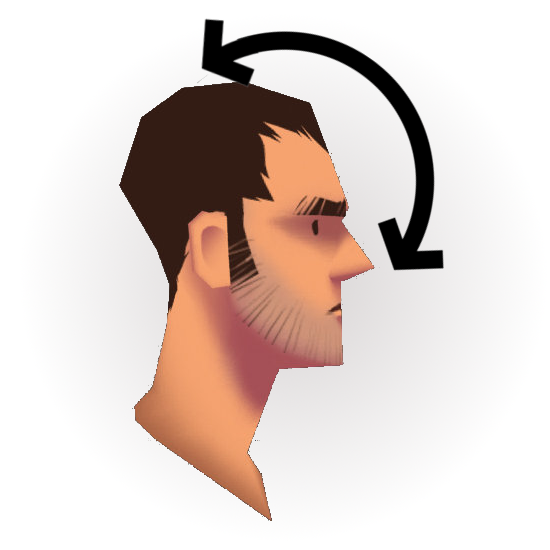
\includegraphics[width=0.95\textwidth]{figuras/pitch.png}
		\caption{rotação vertical (\textit{pitch}).}
		\label{fig:headmotion_pitch}
	\end{subfigure}
	\caption{Movimentos de rotação da cabeça do operador.}
	\fonte{\citeonline{kieranlampert2019} Modificado}
	\label{fig:headmotion}
\end{figure}

Os movimentos indicados na \autoref{fig:headmotion}, são traduzidos em movimentos \textit{pan} e \textit{tilt} da câmera, como ilustrado na \autoref{fig:cameramotion}.

\begin{figure}[H]
	\centering
	\begin{subfigure}{.5\textwidth}
		
\includegraphics[width=0.90\textwidth]{figuras/Pan1.pdf}
		\caption{visão superior de uma câmera,\newline indicando o movimento horizontal (\textit{pan}).}
		\label{fig:cameramotion_pan}
	\end{subfigure}%
	\begin{subfigure}{.5\textwidth}
		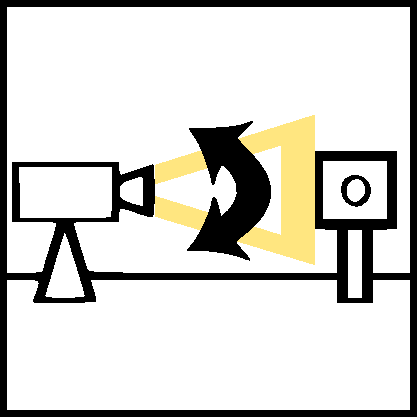
\includegraphics[width=0.90\textwidth]{figuras/Tilt1.pdf}
		\caption{visão lateral de uma câmera,\newline indicando movimento vertical (\textit{tilt}).}
		\label{fig:cameramotion_tilt}
	\end{subfigure}
	\caption{Movimentos da Câmera.}
	\fonte{\citeonline{publicdomain2019} Modificado}
	\label{fig:cameramotion}
\end{figure}

\section{Especificação do Projeto}
\label{sec:especificacao}

O projeto pode ser dividido conceitualmente em duas partes, denominadas por: \textbf{Módulo de Controle de Câmera (MCC)}, o \textit{Raspberry Pi} e \textbf{Módulo de Captura de Movimento (MCM)}, o \textit{smartphone} \textit{Android}. O MCC é responsável por receber os dados de posição através de uma conexão \textit{socket}, converter o sistema de coordenadas, aplicar um filtro para evitar o acionamento desnecessário dos motores, impedindo o aquecimento, e acionar os servos. O MCM é responsável por configurar os sensores de localização disponíveis no \textit{smartphone}, aplicar os filtros necessários para minimizar ruídos na coleta de dados, configurar automaticamente uma conexão \textit{socket} com MCC, através de uma busca na rede, e enviar dados das coordenadas. \par

\begin{figure}[H]
	\centering
	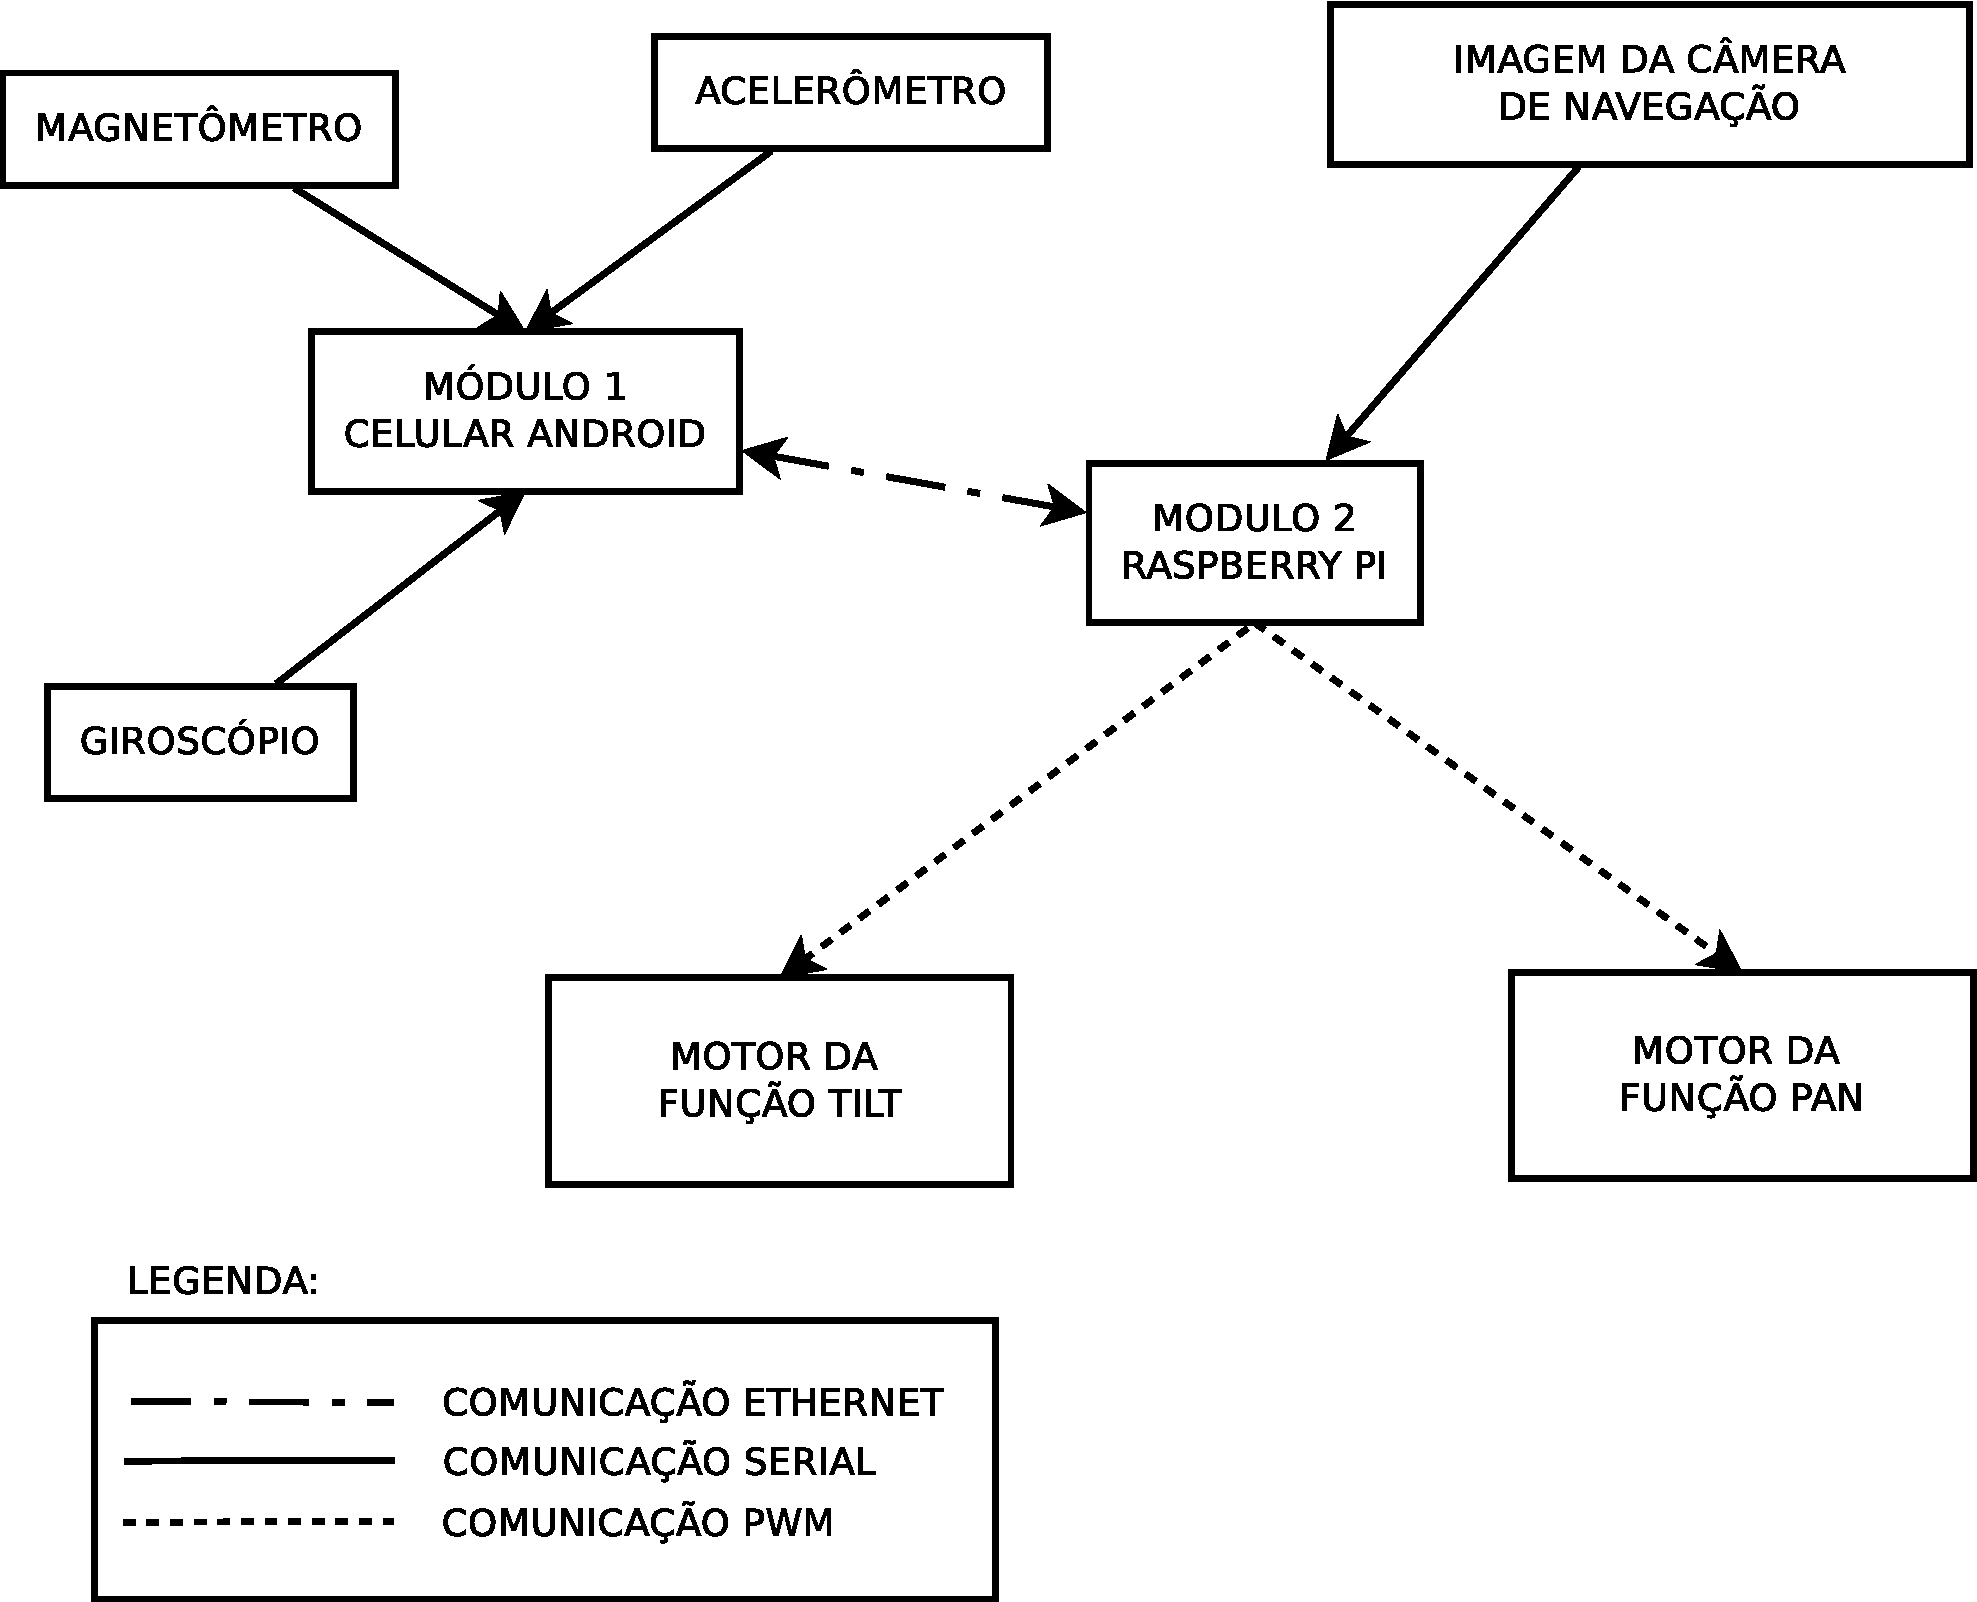
\includegraphics[trim={6cm 3cm 5cm 3cm},clip,width=0.8\textwidth]{figuras/diagrama-modulos-eps-converted-to.pdf}
	\caption{Diagrama de blocos da comunicação entre os principais componentes da solução}
	\label{fig:diagrama_blocos}
\end{figure}

A \autoref{fig:diagrama_blocos} ilustra a comunicação entre os módulos, sensores e atuadores. Os sensores estão embarcados no \textit{smartphone} e não serão controlados separadamente, sendo automático o seu acionamento. O sistema operacional \textit{Android} fornece uma abstração para o hardware, e portanto, não será necessário configurar os sensores manualmente.

\subsection{Módulo de Controle de Câmera (MCC)}
\label{subsec:modconcam}

O Módulo de Controle de Câmera consiste em um SoC \textit{Raspberry Pi} 1 modelo B, que possui um processador ARM de 700MHz, 512Mb de memória RAM, 26 pinos de propósito geral (GPIO), duas portas USB e uma porta Ethernet. O MCC tem as seguintes responsabilidades:

\begin{itemize}
	\item Responder requisições \textit{broadcast} particulares, que identificam o MCM;
	\item Receber dados de posição de sensores;
	\item Filtrar os dados recebidos para evitar acionamento desnecessário dos motores;
	\item Traduzir coordenadas dos sensores para coordenadas das câmeras;
	\item Acionar dois servo motores de acordo coordenadas recebidas;
	\item Iniciar o serviço de \textit{stream} de vídeo;
	\item Finalizar o serviço de \textit{stream} de vídeo;
	\item Calibrar a posição da câmera (salvar posição corrente e usar esse dado para os próximos movimentos).
\end{itemize}

\subsection{Módulo de Captura de Movimento (MCM)}
\label{subsec:modcapmov}

O Módulo de Captura de Movimento é um \textit{smartphone} \textit{Android} Motorola G6 com processador, de arquitetura ARM, modelo \textit{Qualcomm} \textit{Snapdragon 450}, com 8 núcleos (Octa-Core), com \textit{clock} de 1,8 GHz, 3GB de memória RAM, conectividade \textit{Wi-Fi}, que possui os seguintes sensores: acelerômetro, magnetômetro, giroscópio, proximidade, luz ambiente e leitor de impressão digital. O MCM é responsável por:

\begin{itemize}
	\item Enviar requisição \textit{broadcast} especial para detectar o MCC;
	\item Conectar no MCC;
	\item Configurar a orientação do dispositivo em relação aos eixos de referência (\autoref{fig:axisdevice} e \autoref{fig:axisglobe});
	\item Coletar dados dos sensores de movimento;
	\item Aplicar filtros nos dados obtidos dos sensores;
	\item Enviar coordenadas para o MCC;
	\item Mostrar vídeo capturado pela câmera do MCC em formato \textit{stereo};
	\item Mostrar informações pertinentes ao estado do MCC, como o endereço IP (\textit{Internet Protocol}) configurado.
\end{itemize}

\section{Montagem do Protótipo}
\label{sec:assemprototipo}

O protótipo foi construído usando uma PSU (\textit{Power Supply Unit}) de computador de mesa, padrão ATX (\textit{Advanced Technology eXtended}), como fonte de alimentação e suporte de montagem para todos os componentes, com exceção do \textit{smartphone}.\par

Foi usada cola quente para fixar na fonte de alimentação (PSU), usada como base de apoio dos componentes, o \textit{Raspberry Pi}, corpo de montagem da câmera com motores servos (suporte articulado) e um ponto de acesso sem fio, que fornece a infra-estrutura de rede para o projeto. \par

O suporte dos servo motores e da câmera é uma estrutura moldada em plástico, ilustrado na \autoref{fig:basedesmontada}, que precisa ser montada com parafusos. A posição de descanso dos motores (centro de curso) precisa ser regulada neste momento, não sendo possível modificar está posição facilmente depois que o suporte estiver montado, ilustrado na \autoref{fig:basemontada}.\par

\begin{figure}[H]
	\centering
	\begin{subfigure}{.5\textwidth}
		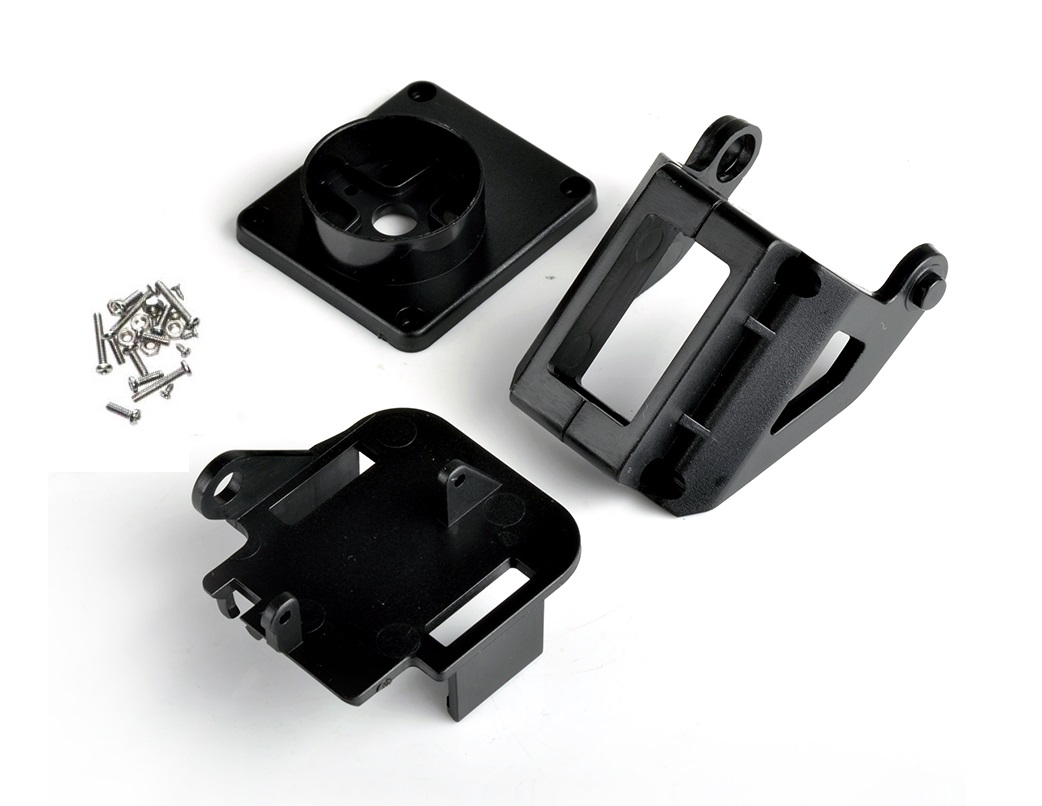
\includegraphics[width=0.95\textwidth]{figuras/base2.jpg}
		\caption{Componentes do suporte.}
		\label{fig:basedesmontada}
	\end{subfigure}%
	\begin{subfigure}{.5\textwidth}
		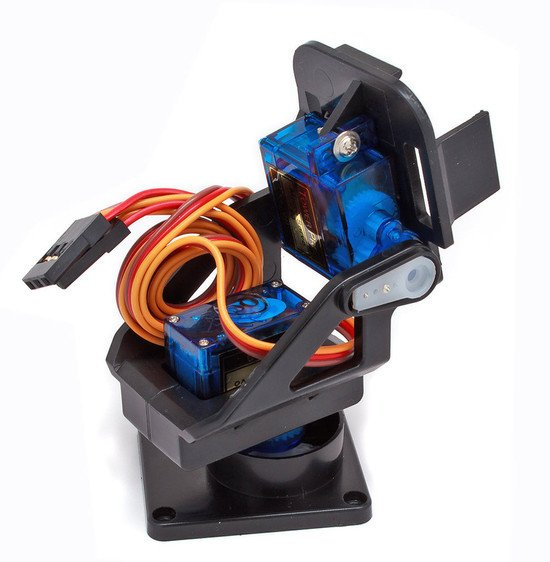
\includegraphics[width=0.75\textwidth]{figuras/base3.jpg}
		\caption{Montagem com motores.}
		\label{fig:basemontada}
	\end{subfigure}
	\caption{Base de suporte para motores e câmera.}
\end{figure}

\subsection{Circuito de Teste para Servo Motor}
\label{subsec:servotester}

Com a intenção de testar os motores e preservar o \textit{Raspberry Pi} (um dispositivo menos tolerante a falhas, quando se trata de níveis de tensão nos pinos GPIO), foi desenvolvido um circuito gerador de sinal PWM (\textit{Pulse width modulation}), também conhecido como \textbf{\textit{driver} PWM}, ilustrado na \autoref{fig:pwmtestcircuit}. O circuito permitia ajustar tanto a frequência do sinal quanto a largura dos pulsos, através de ajustes no potenciômetro POT3 e de um resistor que substituiu os potenciômetros POT1 e POT2 no circuito real, implementado na \textit{breadboard}. Utilizando o circuito, foi possível identificar a posição central dos motores e verificar sua estabilidade, enquanto se variava a frequência do sinal. O drive foi montado usando o circuito integrado NE555, um componente eletrônico bastante usado em aplicações que envolve temporização, geração de pulso e PWM. \par

\begin{figure}[H]
	\centering
	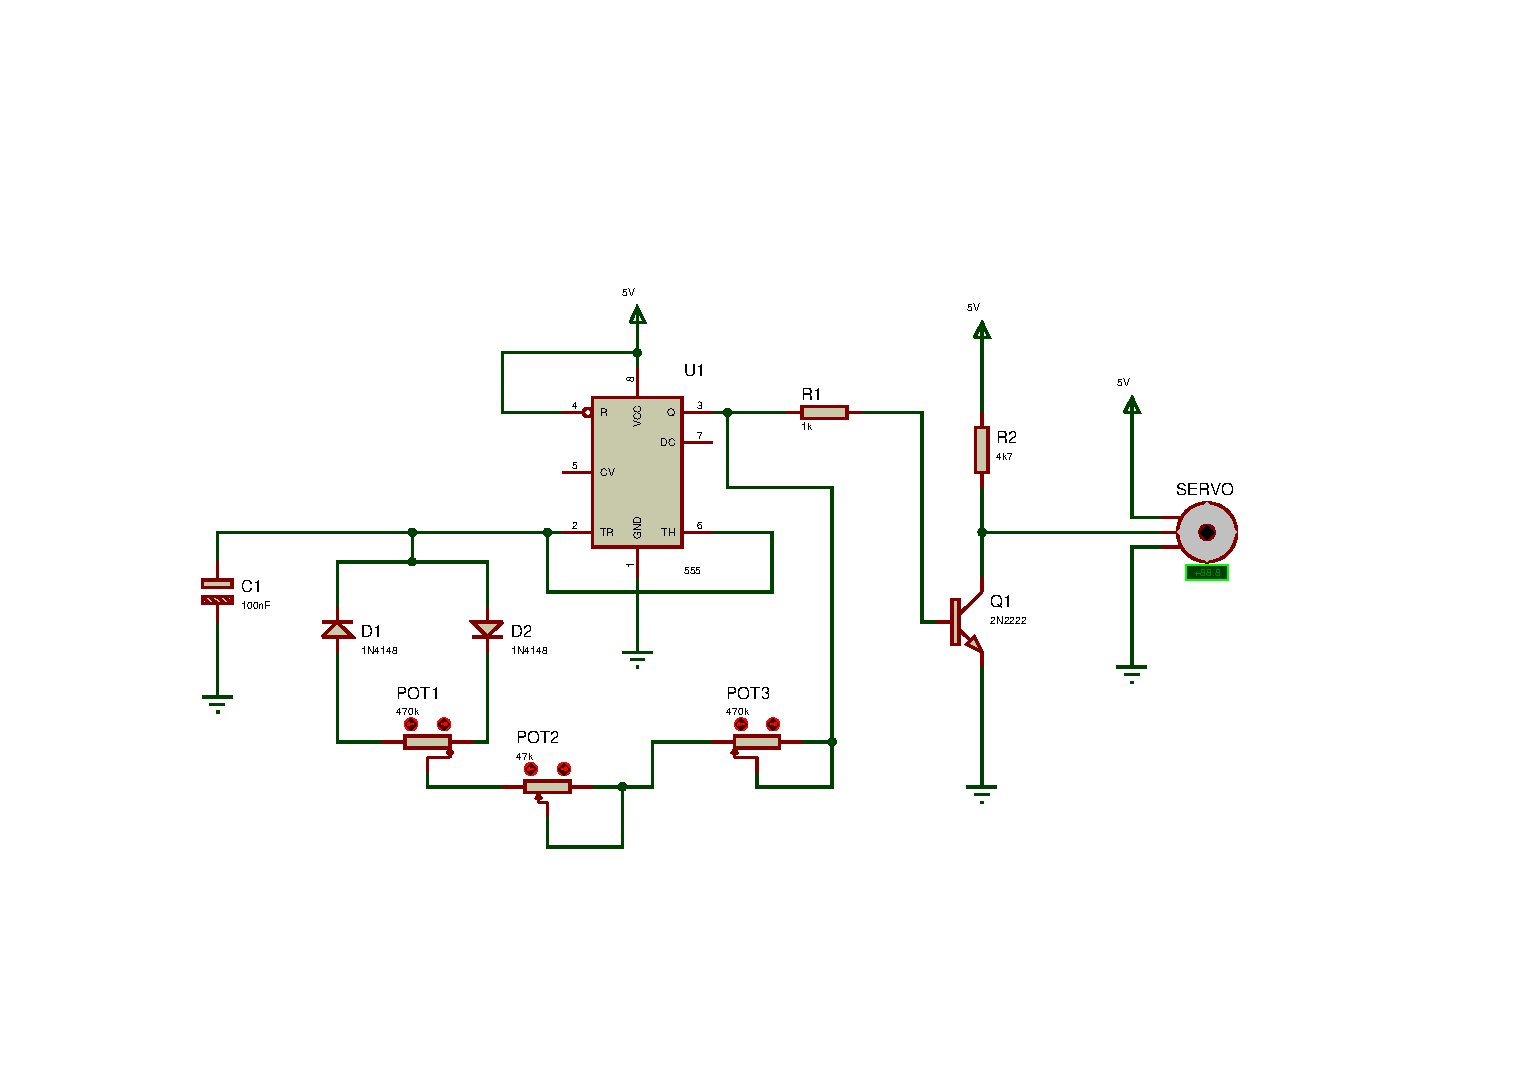
\includegraphics[trim={2.5cm 3cm 4cm 5cm},clip,width=1\textwidth]{figuras/pwm2.pdf}
	\caption{\textit{Driver} PWM de teste.}
	\label{fig:pwmtestcircuit}
\end{figure}

Ativando individualmente os motores com o \textit{driver} construído e com o auxílio de um osciloscópio, foi possível notar que os motores operam de forma estável com pulsos gerados numa frequência de 50Hz, e que é possível controlar a sua posição variando a largura do pulso entre valores próximos a 1ms, posição de ângulo $180\degree$ (ângulo máximo), e valores próximos a 2ms, posição de ângulo $0\degree$ (ângulo mínimo), como ilustrado na \autoref{fig:pwmservo}. Foi possível observar também, que existe uma correspondência linear entre a largura do pulso e a posição angular do eixo do motor, sendo assim, a posição de repouso ou centro, pode ser alcançada com uma largura de pulso próximo a 1,5 milissegundos. 

\begin{figure}[H]
	\centering
	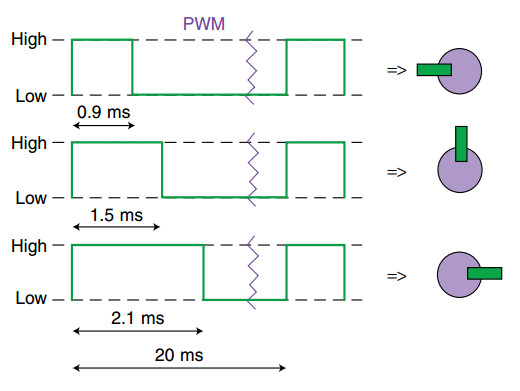
\includegraphics[width=0.7\textwidth]{figuras/pwm_servo.jpg}
	\caption{Posição do eixo do motor em função da largura de pulso PWM.}
	\fonte{\citeonline{pinckney2006pulse}}
	\label{fig:pwmservo}
\end{figure}

\subsection{Circuitos de Acionamento dos Servo Motores}
\label{subsec:servomotorcircacionamento}

Para conectar os motores ao módulo de câmera \textit{Raspberry Pi}, foi necessário construir um circuito de acionamento dos motores, que consiste em dois transistores bipolares de junção (BJT 2N2222), um para cada motor, configurados no modo emissor-comum, funcionando como um interruptor acionado pelo sinal PWM gerado pelos pinos GPIO do \textit{Raspberry Pi}. A fonte do sinal PWM foi ligada ao terminal base do transistor através de um resistor de 1K$\Omega$, com a função de limitador de corrente $I_b$ e a via de sinal do motor, foi conectada ao terminal coletor do transistor juntamente a uma fonte de 5V através de um resistor de 10K$\Omega$, responsável por limitar a corrente $I_c$, máxima quando o transistor está ativado, como ilustrado no circuito da \autoref{fig:circprotecao}.\par

Esse circuito foi construído numa mini \textit{breadboard} e tem o objetivo proteger o \textit{Raspberry Pi}, evitando o consumo excessivo de corrente (mais que 15mA), ou uma possível corrente de retorno para um dos pinos GPIO, numa eventual falha do circuito interno de controle dos motores. Como o circuito de proteção inverte o sinal PWM, foi necessário gerar um sinal invertido no MCC, para que esse fosse invertido novamente pelo circuito de proteção e assim chegar como devido ao circuito de controle interno do motor.\par

\subsection{Circuitos de Alimentação dos Servo Motores}
\label{subsec:servomotorcircalimentacao}

A alimentação dos motores é fornecida por um outro circuito composto por um regulador linear de tensão, o LM7805, e dois capacitores, ilustrado na \autoref{fig:circfonte}, que reduz a tensão de 12V, fornecida pela PSU, pra 5V. A linha de 12V foi usada para isolar as fontes de alimentação dos motores e do \textit{Raspberry Pi}, para evitar ruídos causados pelo acionamento dos motores.

\begin{figure}[H]
	\centering
	\begin{subfigure}{.5\textwidth}
		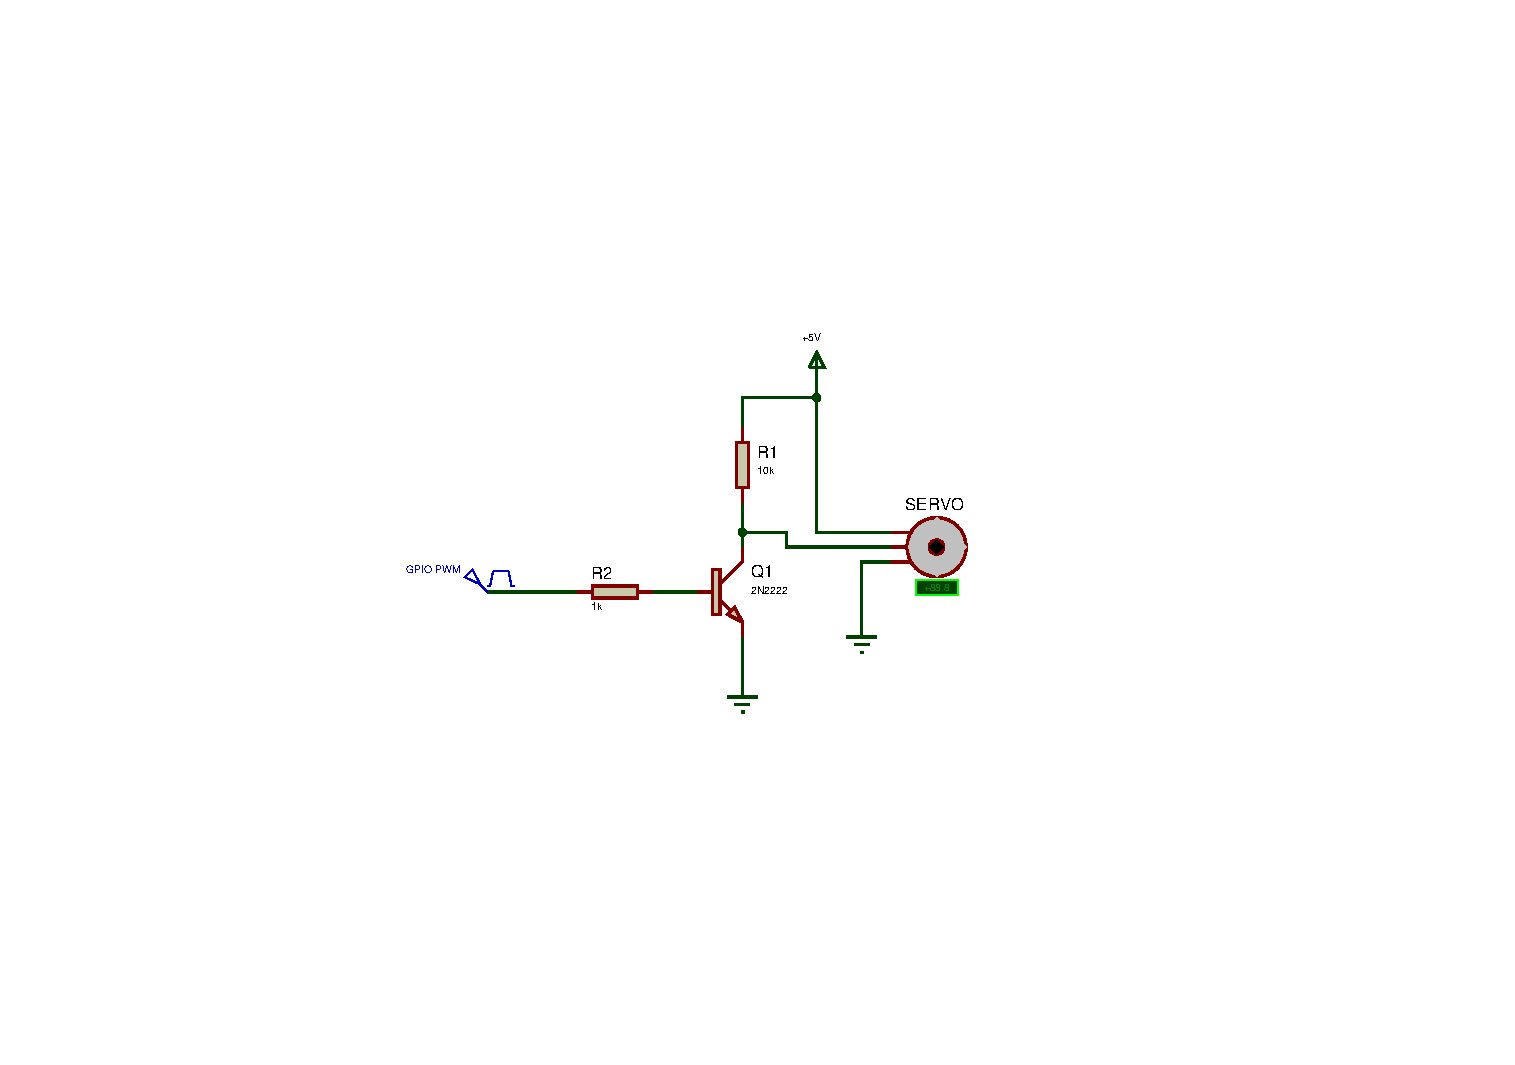
\includegraphics[trim={6.5cm 5cm 9cm 5cm},clip,width=0.9\textwidth]{figuras/circ_acionamento.pdf}
		\caption{Acionamento de motores.}
		\label{fig:circprotecao}
	\end{subfigure}%
	\begin{subfigure}{.5\textwidth}
		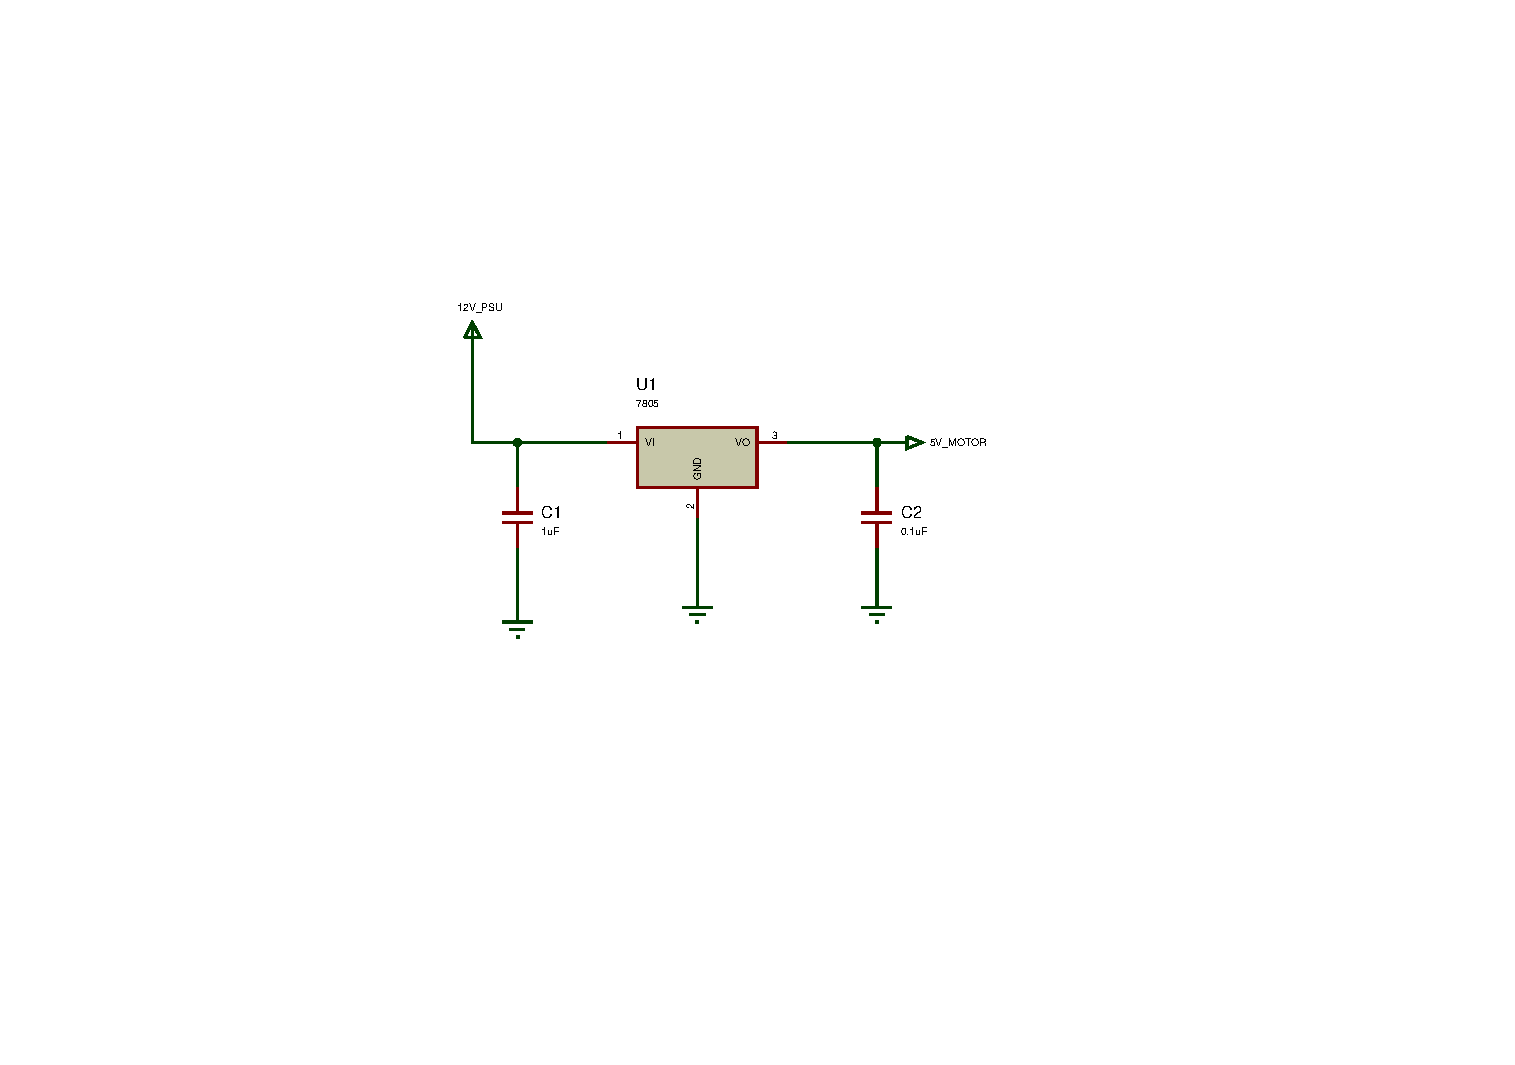
\includegraphics[trim={6.5cm 5cm 8.5cm 4cm},clip,width=0.9\textwidth]{figuras/fonte_motores.pdf}
		\caption{Regulador de tensão.}
		\label{fig:circfonte}
	\end{subfigure}
	\caption{Circuitos usados pelos motores.}
\end{figure}

\subsection{Construção do Módulo de Controle de Câmera - MCC}
\label{subsec:assemmodconcam}

O MCC é responsável por acionar os motores, usados para movimentar a câmera, e iniciar um serviço de \textit{stream} de mídia, que disponibiliza na rede usando um protocolo de tempo real, as imagens capturadas pela câmera.\par

O \textit{software} de controle foi construído, usando a linguagem C, para receber valores de coordenadas enviados por uma conexão \textit{socket} e acionar os motores.\par

O MCC possui dois modos de operação, um modo de produção, que opera consumindo recursos mínimos de memória e processador, e um modo de depuração/teste, habilitado através da diretiva \textbf{\textit{\#define TEST\_DISPLAY}} ou diretamente pelo \textit{script} \textit{Makefile} passando o parâmetro \textbf{\textit{CFLAGS=-DTEST\_DISPLAY}}.
\begin{figure}[H]
	\centering
	\begin{subfigure}{.5\textwidth}
		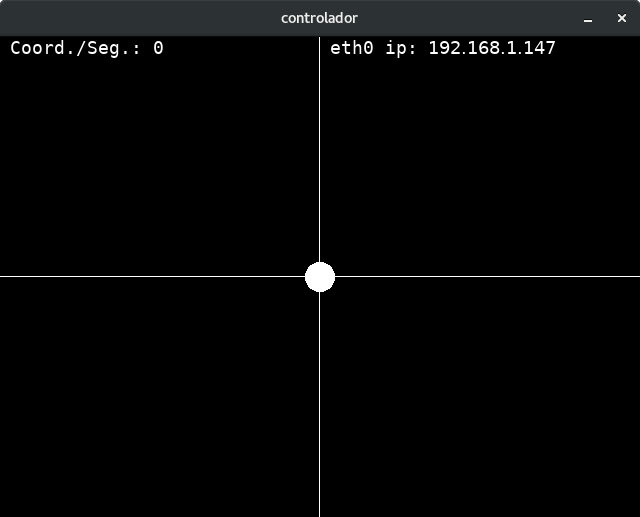
\includegraphics[width=0.95\textwidth]{figuras/controlador.jpg}
		\caption{iniciado.}
		\label{fig:controlador_teste}
	\end{subfigure}%
	\begin{subfigure}{.5\textwidth}
		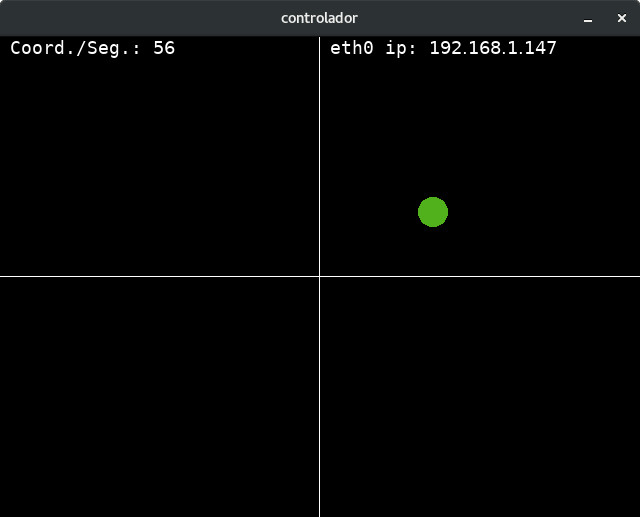
\includegraphics[width=0.95\textwidth]{figuras/controlador2.jpg}
		\caption{gerando posição com o click do mouse.}
		\label{fig:controlador_teste_coordenada}
	\end{subfigure}
	\caption{Captura de tela de depuração e teste dos motores do software de controle.}
\end{figure}

\subsection{Interface de Depuração / Testes}
\label{subsec:iterfacedepuracao}

No modo de depuração, é mostrada uma tela com um painel preto e quatro quadrantes indicando a posição da câmera, através de um ponto branco (localizado no centro dos quadrantes, quando o programa inicia); um indicador, contendo a contagem de coordenadas recebidas por segundo (no canto superior esquerdo) e o endereço IP que está associado a interface de rede do \textit{Raspberry Pi} (no canto superior direito), ilustrado na \autoref{fig:controlador_teste} e na \autoref{fig:controlador_teste_coordenada}. \par

Através dessa interface, é possível simular posições da câmera usando o mouse. Para isso, o ponto branco deve ser clicado e arrastado para uma posição qualquer dos quadrantes. Ao arrastar e soltar o ponto branco, uma coordenada relativa a posição do ponto na tela é calculada e enviada para os motores, ilustrado na \autoref{fig:controlador_teste_coordenada}.\par

Quando o ponto é movido no sentido horizontal, o motor horizontal é acionado, e de forma semelhante, quando o ponto se move na direção do eixo vertical, o motor vertical é acionado.\par

As coordenadas do ponto branco são capturadas em relação a sua posição, em \textit{pixels} horizontais e verticais, dentro do painel preto, sendo a coordenada (0;0) a menor possível, localizada no canto superior esquerdo, ilustrado na \autoref{fig:sistcoord0x0}, e a coordenada (640; 480) a maior possível, localizada no canto inferior direito do painel preto, ilustrada na \autoref{fig:sistcoord100x100}.\par

Conforme explicado na \autoref{sec:servomotor}, os motores servos deslocam seu eixo de acordo com a largura do pulso, enviado para seu controlador interno. Entretanto, as coordenadas simuladas pela interface de depuração e as que são recebidas do módulo \textit{Android}, não possuem a informação de largura de pulso ou quantidade de ângulos que determinado motor deve ser movimentado. Para resolver esse problema, foi proposto um sistema de posição independente da quantidade de \textit{pixels}, largura de pulso ou ângulos.\par

\begin{figure}[H]
	\centering
	\begin{subfigure}{.5\textwidth}
		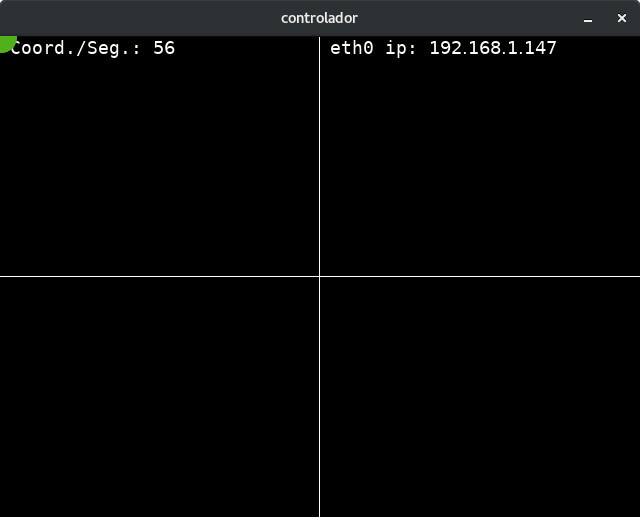
\includegraphics[width=0.95\textwidth]{figuras/controlador0x0.jpg}
		\caption{coordenada mínima}
		\label{fig:sistcoord0x0}
	\end{subfigure}%
	\begin{subfigure}{.5\textwidth}
		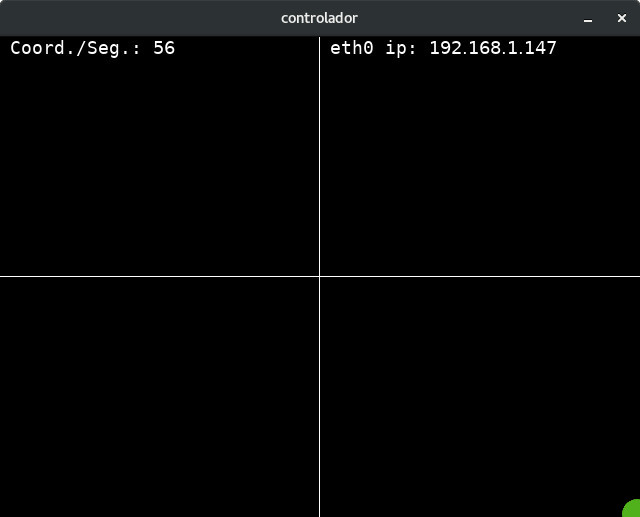
\includegraphics[width=0.95\textwidth]{figuras/controlador100x100.jpg}
		\caption{coordenada máxima}
		\label{fig:sistcoord100x100}
	\end{subfigure}

	\begin{subfigure}{.5\textwidth}
	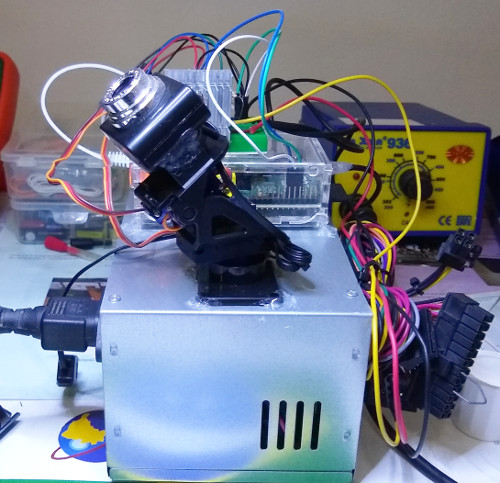
\includegraphics[width=0.95\textwidth]{figuras/camera0x0.jpg}
	\caption{reflexo da coordenada mínima na câmera}
	\label{fig:camera0x0}
	\end{subfigure}%
	\begin{subfigure}{.5\textwidth}
		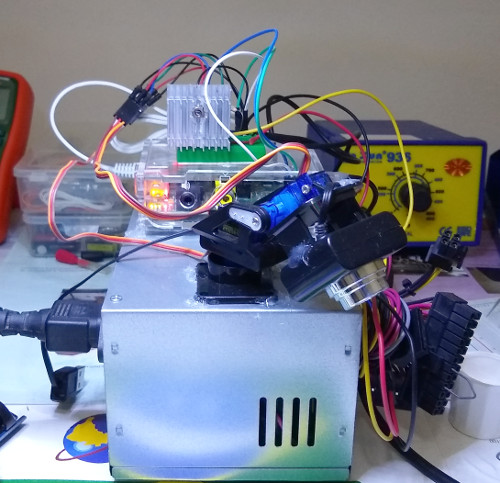
\includegraphics[width=0.95\textwidth]{figuras/camera100x100.jpg}
		\caption{reflexo da coordenada máxima na câmera}
		\label{fig:camera100x100}
	\end{subfigure}


	\begin{subfigure}{.5\textwidth}
		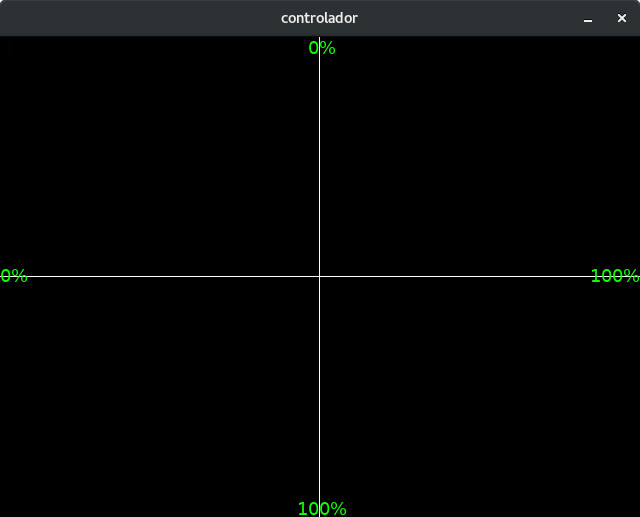
\includegraphics[width=0.95\textwidth]{figuras/controlador-values.jpg}
		\caption{orientação dos eixos.}
		\label{fig:sistcoord}
	\end{subfigure}
	\caption{Sistema de coordenadas proporcional.}
\end{figure}

\subsection{Sistema de Coordenadas}
\label{subsec:sistemacoordenadas}

O sistema de posição proposto é baseado na proporção ou porcentagem máxima do movimento possível (do motor, da cabeça do operador e do mouse no painel do programa de teste). Desse modo, o ângulo máximo que o motor horizontal e a cabeça do operador podem deslocar é $180\degree$, sendo $90\degree$ para a esquerda e $90\degree$ para a direita (partindo-se do ângulo $90\degree$, local de descanso do motor e centro de visão do operador), e está relacionado diretamente ao valor máximo de \textit{pixels} que a componente $x$ da coordenada de posição pode assumir, 640 \textit{pixels}, sendo 320 para a esquerda e 320 para a direita (partindo-se do centro da interface). De forma semelhante, movem-se no eixo vertical, o motor e a cabeça do operador com ângulo máximo de $180\degree$, mudando apenas a quantidade máxima de \textit{pixels} na interface de teste, que nesse caso é 480, sendo 240 para cima e 240 para baixo.\par
A relação entre a largura de pulso enviada para os motores horizontal e vertical, em porcento, é dada respectivamente por:
\begin{equation}
	PWM_H = \frac{TARGET_X \times 100}{WIDTH}
	\label{eq:pwm_screen_h}
\end{equation}

\begin{equation}
	PWM_V = \frac{TARGET_Y \times 100}{HEIGHT}
	\label{eq:pwm_screen_v}
\end{equation}

Sendo $WIDTH = 640$ e $HEIGHT = 480$, a largura e altura do painel de teste; $TARGET_X$ e $TARGET_Y$ a localização real em \textit{pixels} horizontais de verticais do ponto branco indicador.

A \autoref{fig:sistcoord} mostra que o valor dos componentes das coordenadas crescem no sentido esquerda-direita, horizontalmente e, cima-baixo, verticalmente. Como o sistema está expresso em porcentagem, os valores das coordenadas são enviados diretamente para os motores, como será visto adiante, no final da \autoref{subsec:deiverpwm}.\par

Um ajuste foi feito nas coordenadas que são enviadas para o motor servo que movimenta a câmera horizontalmente. Devido a montagem do motor inverter a posição do seu eixo, as coordenadas enviadas pela interface de depuração e pelo MCM foram invertidas. Sendo assim a \autoref{eq:pwm_screen_h} foi ajustada para:

\begin{equation}
	PWM_H = 100 - (\frac{TARGET_X \times 100}{WIDTH})
	\label{eq:pwm_screen_h_inverse}
\end{equation}

Na \autoref{fig:sistcoord0x0}, é possível visualizar o marcador de posição em verde (enquanto o botão esquerdo do mouse está pressionado) na posição (0;0), selecionado manualmente com o mouse, e seu reflexo nos motores, mostrado na \autoref{fig:camera0x0}. O mesmo acontece com o ponto máximo, ilustrado na \autoref{fig:sistcoord100x100} e o reflexo da seleção nos motores, na \autoref{fig:camera100x100}.\par

\subsection{Modo de Demonstração}
\label{subsec:camdemo}

O programa de teste também possui uma função de demonstração, que gera coordenadas de forma automática para os motores servo. Assim, não é necessário escolher uma posição manualmente ou conectar o MCM. A câmera segue o padrão de movimento definido por uma função seno, que varre os limites verticais e horizontais da interface, isto é, o padrão de movimento começa na coordenada (0;50) e oscila como uma senoide até a coordenada (100;50), ilustrado na \autoref{fig:camdemo_inc}. Quando o movimento chega ao limite horizontal, a função é invertida e a câmera volta ao ponto de origem, conforme ilustrado na \autoref{fig:camdemo_dec}. O modo de demonstração pode ser ativado através da diretiva \textit{\textbf{\#define CAMDEMO}} ou diretamente pelo \textit{script} \textit{Makefile} passando o parâmetro \textbf{\textit{CFLAGS=-DCAMDEMO}}.

\begin{figure}[H]
	\centering
	\begin{subfigure}{.5\textwidth}
		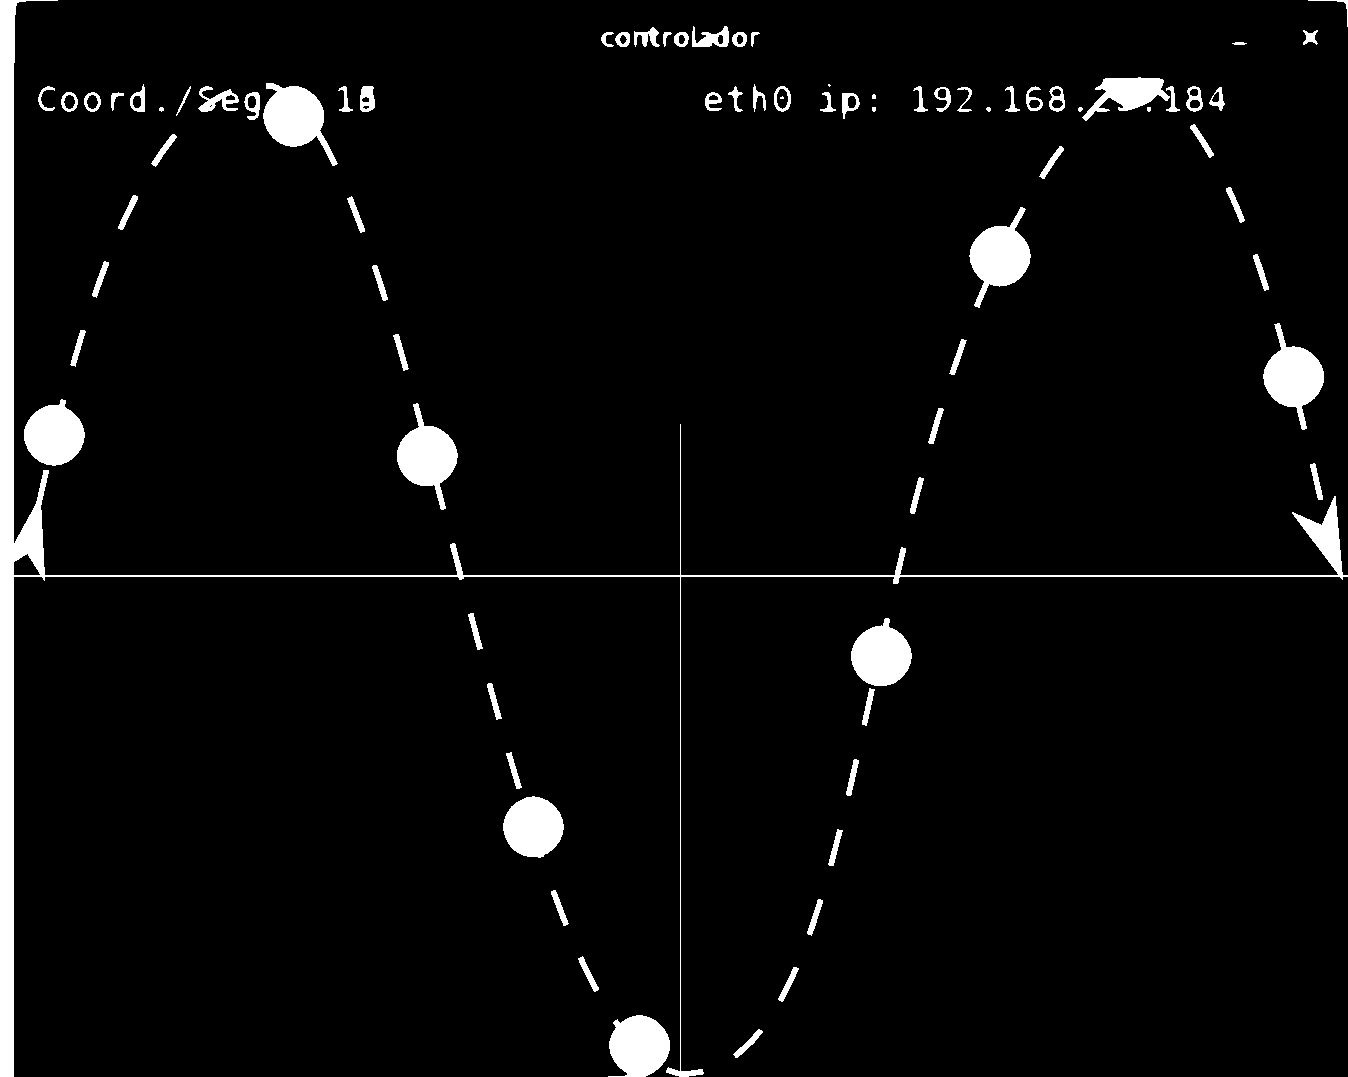
\includegraphics[width=0.95\textwidth]{figuras/camdemo_inc.pdf}
		\caption{movimento crescente}
		\label{fig:camdemo_inc}
	\end{subfigure}%
	\begin{subfigure}{.5\textwidth}
		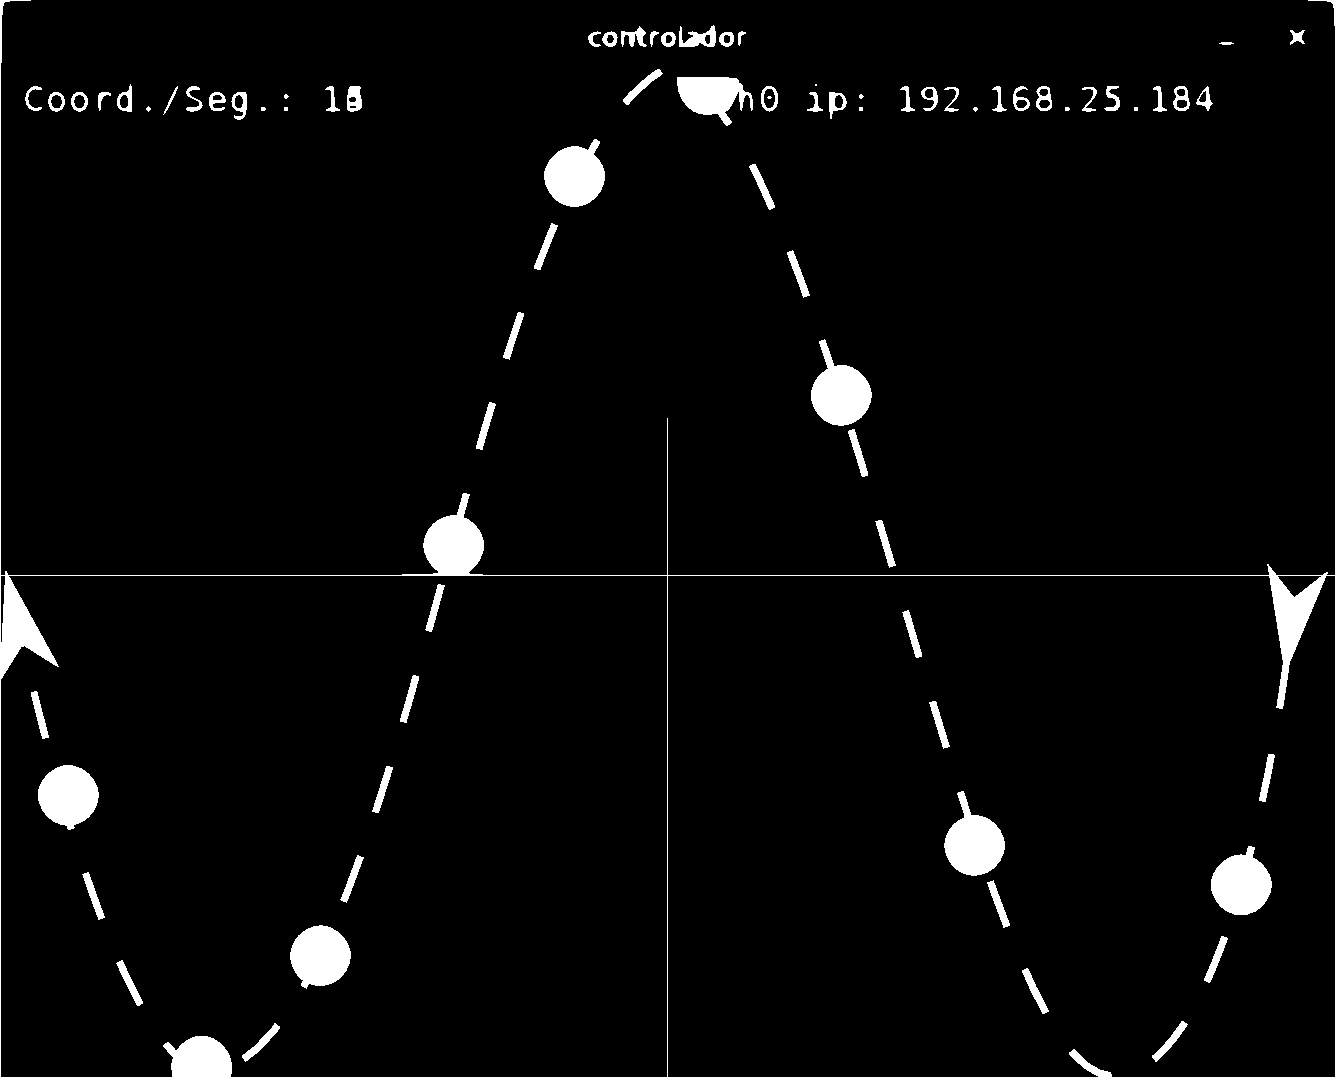
\includegraphics[width=0.95\textwidth]{figuras/camdemo_dec.pdf}
		\caption{movimento decrescente}
		\label{fig:camdemo_dec}
	\end{subfigure}
	\caption{Coordenadas geradas pela função \textit{CAMDEMO}}
	\label{fig:camdemo}	
\end{figure}

\subsection{Driver PWM}
\label{subsec:deiverpwm}

A geração de PWM pode ser realizada através de software ou hardware, usando um dispositivo especializado, implementado dentro do processador.\par

Testes foram feitos no início do projeto na expectativa de gerar um sinal PWM adequado via software, usando a biblioteca \textbf{RPi.GPIO}, escrita em \textit{python}, já que a ideia inicial era escrever todos os módulos, inclusive o programa de testes, em \textit{python}. Entretanto, os resultados não foram satisfatórios. Os pulsos PWM gerados pela biblioteca não mantinham a frequência e nem a largura do pulso, causando um movimento errático dos motores. A partir desse teste, optou-se por utilizar a linguagem de programação C, nas bibliotecas e ao escrever o código dos softwares utilizados no \textit{Raspberry Pi}.\par

Outros testes foram feitos com uma biblioteca chamada \textbf{WiringPi}, escrita usando a linguagem C. A biblioteca não oferecia um bom suporte para PWM, sendo mais utilizada para controle geral dos pinos de propósito geral do \textit{Raspberry Pi}, e portanto foi descartada.\par

A biblioteca \textbf{bcm2835} também foi testada. Observou-se que é uma biblioteca muito extensa e oferece suporte aos diversos dispositivos de hardware como SPI, I2C e PWM, disponíveis no \textit{Raspberry Pi}. Entretanto, por não possuir uma documentação intuitiva e devido a sua complexidade associada ao curto tempo para a conclusão do projeto, sua utilização também foi descartada.\par

Por fim, o método utilizado para gerar um PWM estável, de forma rápida e confiável, foi através do utilitário \textbf{ServoBlaster}, um software que provê uma interface de controle do \textit{driver} PWM, via árvore de dispositivos do sistema operacional \textit{Linux}. Sendo assim, através de um dispositivo localizado em \textbf{/dev/servoblaster}, foi possível gerar sinais PWM estáveis, para múltiplos pinos do \textit{Raspberry Pi}.\par 

Para acionar o \textit{driver} PWM, basta abrir o dispositivo \textbf{/dev/servoblaster}, como um arquivo e escrever os comandos de acionamento dos motores.\par

O utilitário \textbf{ServoBlaster} é instalado como um serviço no sistema operacional e fica esperando comandos serem escritos no dispositivo \textbf{/dev/servoblaster}, criado durante a instalação. Os comandos de acionamento dos servos são intuitivos e não é necessário conhecimento aprofundado em servo motores ou na eletrônica por trás da geração de PWM. Como exemplo, para mover um motor servo qualquer, conectado a um pino $X$ do \textit{Raspberry Pi}, para a posição $90\degree$, seu centro ou ponto de descanso, basta usar um emulador de terminal, como o \textit{bash}, e digitar o comando \textbf{echo X=50\% > /dev/servoblaster}. Para mover o mesmo motor para sua posição inicial, ou $0\degree$, basta digitar \textbf{echo X=0\% > /dev/servoblaster}, e assim sucessivamente para qualquer ângulo $\theta$, sendo $0 \le \theta \le 180$.\par

O MCC usa o utilitário \textit{servoblaster} conforme descrito anteriormente, contudo acessa o dispositivo \textbf{/dev/servoblaster} diretamente, isto é, através das funções de manipulação de arquivo (\textit{open} e \textit{write}), fornecidas pela API C básica do \textit{Linux}, a \textit{stdlibc}.

\subsection{Servidor de Imagens}
\label{subsec:mediaserver}

O MCC também é responsável por enviar as imagens da câmera, em tempo real, para o MCM. Com esse objetivo, testes foram feitos com a \textit{GStreamer}, uma biblioteca bastante utilizada na criação e manipulação de som e vídeo no ambiente \textit{Linux}. Contudo, devido a uma incompatibilidade do sistema operacional utilizado no \textit{Raspberry Pi} e a biblioteca, a \textit{GStreamer} não foi adotada.\par

O VLC (\textit{VideoLAN Client}), um \textit{player} bastante difundido e multi-plataforma, com suporte a vários formatos de som e imagem, capaz de realizar \textit{stream}, usando protocolos de tempo real, em modo \textit{headless} (sem carregar uma interface gráfica, via linha de comando), foi testado também. Entretanto, seu uso foi descartado por utilizar demasiadamente o processador (por volta dos 97\% de CPU e 71MB da memória RAM), e isso possivelmente causaria comportamentos indesejados no controle dos motores.\par

Testes foram realizados também com o \textit{FFmpeg}, um utilitário multi-plataforma usado em manipulações de som e imagem, bastante versátil, com suporte a um grande número de \textit{codecs} e capacidade para realizar \textit{stream} de áudio e vídeo. Esse software foi recompilado para o \textit{Raspberry Pi} com o objetivo de ativar seu suporte ao \textit{codec} de vídeo \textbf{h264\_omx}, implementado em hardware, no chip de silício que contém o processador e todos os periféricos do \textit{Raspberry Pi}, visando reduzir o uso do processador para tarefas de decodificação do vídeo. Por apresentar melhor desempenho (em média 70\% do uso do CPU e 46MB de memória RAM), esse utilitário foi usado para enviar o vídeo para o MCM.



\subsection{Construção do Módulo de Captura de Movimento - MCM}
\label{subsec:assemmodcapmov}

O MCM é responsável por obter, filtrar e enviar coordenadas relativas a posição da cabeça do operador, para o MCC. O módulo é constituído pelo \textit{smartphone} \textit{Android}, um conjunto de sensores embutidos no celular, capazes de fornecer dados relativos a orientação com uma boa acuracidade, e é controlado por um software programado em \textit{Java}, que possui uma interface de operação intuitiva, ilustrado na \autoref{fig:móduloandroid}. \par

O programa de captura de coordenadas pode ser resumido basicamente em quatro partes principais: \textbf{coleta de dados} de posição da cabeça do operador; \textbf{envio de coordenadas}; \textbf{interação com o operador} (interface do usuário); e \textbf{exibição do vídeo} capturado pela câmera. Que serão detalhadas adiante, iniciando-se pela  interface com o usuário.\par


\begin{figure}[H]
	\centering
	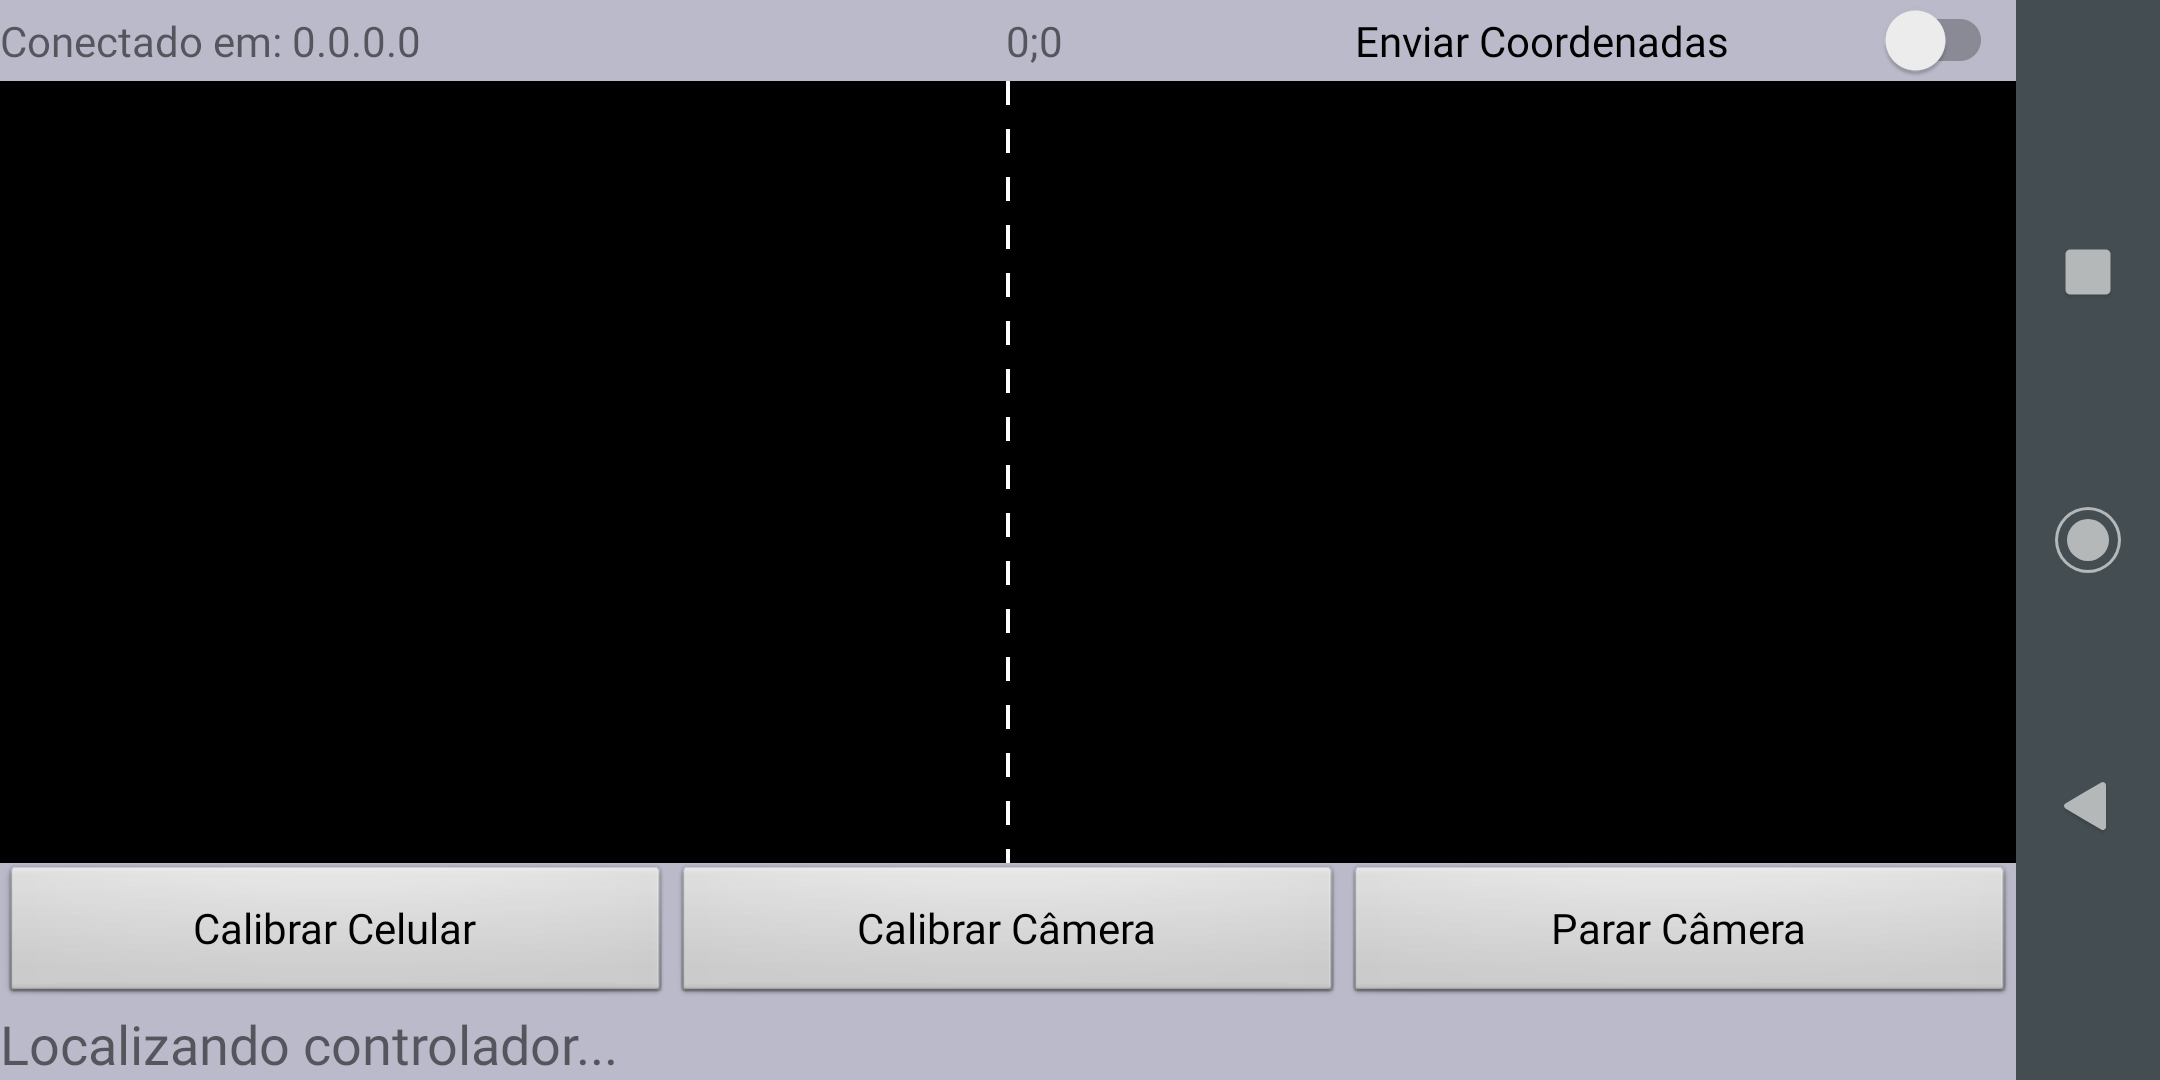
\includegraphics[width=1\textwidth]{figuras/modulo_android_1.png}
	\caption{Interface do Módulo de Captura de Movimento.}
	\label{fig:móduloandroid}
\end{figure}

\subsection{Interface do Usuário / Operador}
\label{subsec:interfaceusuariooperador}

A captura de tela da interface do MCM, ilustrada na \autoref{fig:móduloandroid}, mostra uma série de componentes visuais, que trazem informações pertinentes ao funcionamento do sistema e permitem interagir remotamente com o MCC. \par

O \textbf{indicador de conexão}, localizado no canto superior esquerdo da interface, indica a qual endereço IP está associado ao servidor, responsável por controlar os motores que movimentam a câmera, e ao mesmo tempo disponibilizam as imagens capturadas. Quando o valor mostrado é \textbf{0.0.0.0}, significa que está desconectado de um servidor e não será possível enviar coordenadas ou receber imagens.\par

O \textbf{indicador de coordenadas}, localizado na parte central superior da interface, indica qual coordenada está sendo capturada, em tempo real, pelos sensores de movimento do celular. Seu formato é semelhante a uma coordenada cartesiana, isto é, a componente $x$ seguida pela componente $y$ e separada por um "ponto e vírgula". Esse indicador mostra pontos do sistema de coordenadas proposto na \autoref{subsec:assemmodconcam}. Desse modo, a coordenada \textbf{(50;50)} é equivalente ao centro da interface de depuração.\par

No canto superior direito da interface, se encontra o \textbf{controle de envio de coordenada}, uma chave do tipo \textit{on-off} que somente é habilitada quando o Módulo de Captura de Movimento está conectado a um servidor de controle de câmera. Quando a chave está na posição \textit{on}, ou ativada, as coordenadas são enviadas para o servidor de controle de câmera.\par

Ao centro da interface, numa área em cor preta, está localizado o \textbf{painel de imagens}. Este é o local onde as imagens da câmera são mostradas quando recebidas do módulo de controle de câmera. O painel de imagens é dividido verticalmente ao centro em duas porções, indicado pela linha tracejada em cor branca.\par

A divisão existe em decorrência do sistema de vídeo \textit{stereo} simulado, onde uma única imagem enviada pelo módulo de controle de câmera é duplicada e manipulada, de forma a criar um efeito \textit{parallax}, isto é, criar a sensação de que existem duas fontes de vídeo (duas câmeras), capturando imagens de um mesmo objeto a partir de ângulos de visão distintos, trazendo a sensação 3D para o operador.\par

A interface possui uma \textbf{barra de \textit{status}}, localizada na parte inferior, que indica qual tarefa está sendo executada no momento. A barra de \textit{status} mostrada na \autoref{fig:móduloandroid} indica que o MCM está buscando o MCC.\par

\subsection{Mecanismo de Busca pelo MCC}
\label{subsec:mecanismobuscamcc}

O mecanismo de busca pelo MCC se dá através do disparo de mensagens em \textit{broadcast} do tipo \textit{User Datagram Protocol}, também conhecido como mensagens UDP, partindo do MCM com um código específico, somente respondida pelo MCC com o seu endereço IP associado. Desse modo, o MCM configura o endereço IP respondido como um serviço de controle válido e habilita o mecanismo de envio de coordenadas.\par

Acima da barra de \textit{status} e abaixo do painel de imagens, está localizado o menu de botões, contendo as funções de \textbf{calibração do celular}, que consiste em salvar as coordenadas referentes a posição atual do celular, usadas posteriormente para calcular uma nova coordenada ajustada, que será enviada para o MCC. A função de \textbf{calibração de câmera} envia uma mensagem de calibração para o MCC, solicitando que a coordenada atual dos servo motores sejam persistidas numa estrutura, para que posteriormente seja usada como referência para movimentar a câmera. Por fim, a função \textbf{Parar/Enviar Câmera} controla o envio de imagens capturadas pelo MCC para o MCM.\par

\subsection{Sistema de Vídeo}
\label{subsec:sistemadevídeo}

Devido a escassez de recursos de hardware no \textit{Raspberry Pi} (processador e memória RAM) para esse tipo de aplicação, associados a qualidade inferior da câmera utilizada no protótipo, a imagem capturada e enviada para o \textit{smartphone} não tem uma boa resolução (320x240 \textit{pixels}). Quando escalonada para preencher a área disponível na interface do celular, resultou numa figura disforme que pouco representava o objeto capturado. Sendo assim, apenas uma imagem está sendo mostrada, em tamanho reduzido e fora de alinhamento com a interface, conforme ilustrado na \autoref{fig:móduloandroid_cam}. Também, devido aos mesmos problemas relacionados ao hardware e qualidade da câmera, existe um atraso de aproximadamente 4 segundos entre as imagens que são coletadas na câmera e as imagens que são exibidas no aplicativo do celular.

\begin{figure}[H]
	\centering
	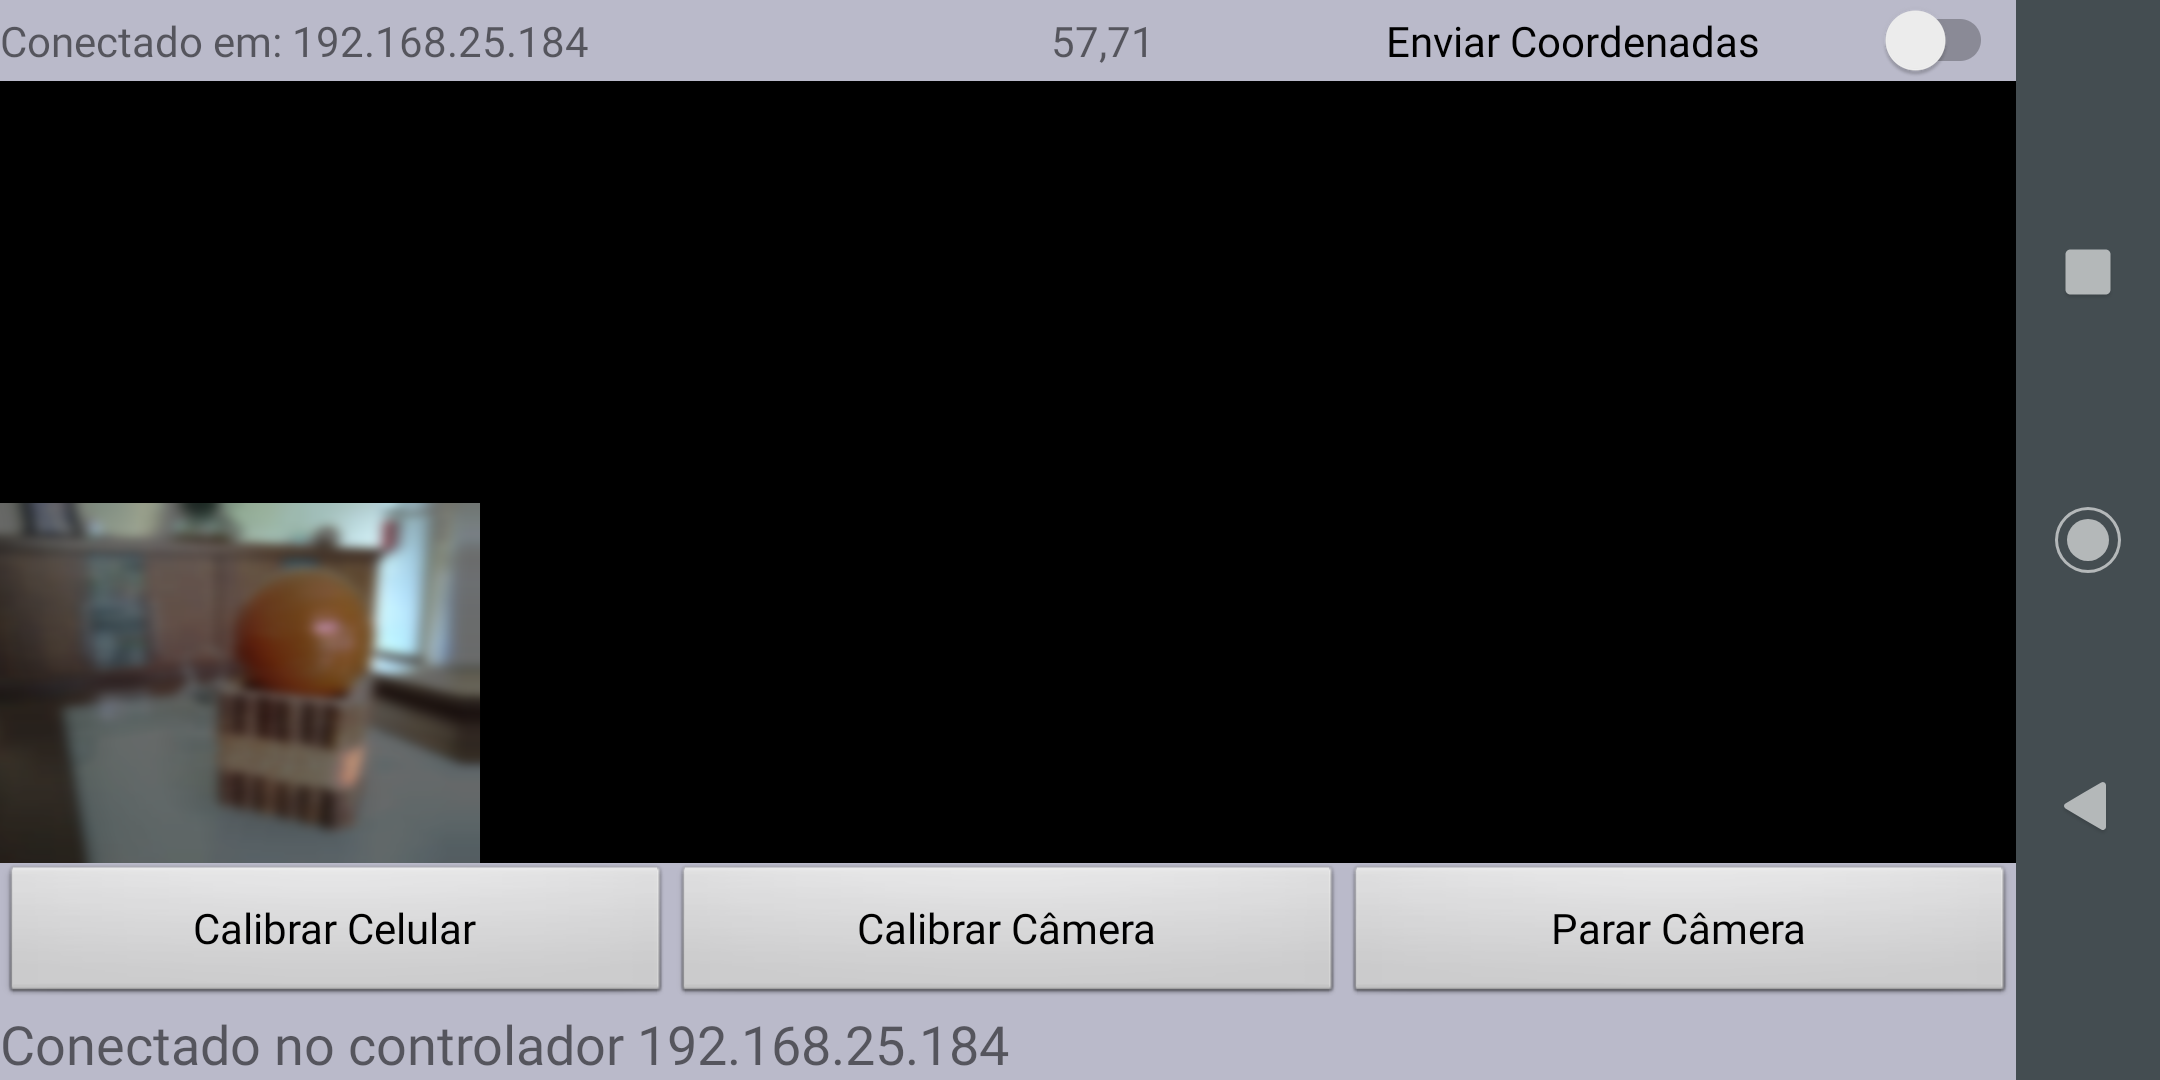
\includegraphics[width=1\textwidth]{figuras/modulo_android_2.png}
	\caption{Imagem da câmera em tamanho original.}
	\label{fig:móduloandroid_cam}
\end{figure}

Para mostrar no celular as imagens capturadas pelo MCC e transmitidas via RTP \textit{(Real Time Protocol)}, foi utilizado a biblioteca do \textit{VLC}, a mesma testada na \autoref{subsec:mediaserver}, que foi recompilada para o sistema operacional \textit{Android} e integrada ao MCM. Essa biblioteca foi selecionada, principalmente por oferecer opções de compatibilidade com o sistema operacional \textit{Android}, como também ser compatível com diversos formatos de vídeo e ter suporte ao \textit{RTP}.\par

\subsection{Sistema de Captura de Coordenadas}
\label{subsec:sistemacapturacoordenadas}

A coleta de dados de movimento acontece a cada 30 milissegundos, através dos eventos de posição fornecidos pela API do sistema operacional \textit{Android}, que simplifica bastante o desenvolvimento de aplicações e abstrai toda a configuração do \textit{hardware} dos sensores e a densa matemática, necessária para converter a leitura de forças exercidas sobre o aparelho e a interações dos vetores aceleração, em uma estrutura de dados que representa numericamente a posição espacial em que se encontra o celular. Contudo, é necessário identificar a orientação do aparelho, ilustrado na \autoref{fig:axisdevice}, em relação ao sistema de eixos do planeta, ilustrado na \autoref{fig:axisglobe} para que a coleta de dados funcione adequadamente.\par

O envio de coordenadas ocorre assim que um evento de posição é disparado. Ou seja, um novo envio de coordenada acontece a cada 30 milissegundos. Supondo que um par de coordenadas em média consuma 5 \textit{bytes} (2 \textit{bytes} para a coordenada $x$, 2 \textit{bytes} para a coordenada $y$ e 1 \textit{byte} para um caractere separador), seriam enviados 167 \textit{bytes} por segundo, desconsiderando o \textit{overhead} do protocolo TCP (\textit{Transmission Control Protocol}), usado para esta finalidade. O consumo da banda de dados, observado pela transmissão das coordenadas, pode ser considerado irrisório para um \textit{link} de 100Mbit/s, atualmente comum em redes do tipo \textit{Ethernet}. Entretanto, visando reduzir os recursos computacionais do celular, e consequentemente economizar bateria, um filtro verifica se houve mudança nas coordenadas antes de enviá-las, reduzindo o uso da banda de dados para aproximadamente 7 \textit{bytes} por segundo (considerando que o MCM está em repouso, na posição de descanso).\par

  
	% RESULTADOS-------------------------------------------------------------------

\chapter{RESULTADOS}
\label{chap:resultados}

Nesse capítulo serão discutidos os resultados globais obtidos com o desenvolvimento do protótipo e será mostrado um teste comparativo entre dois \textit{codecs} de vídeo com a biblioteca \textit{FFmpeg}.\par

\subsection{Resultados Globais}
\label{subsec:resglobais}

De modo geral, o protótipo se comportou conforme o esperado. A captura de movimento da cabeça do operador funcionou de maneira satisfatória e os motores responderam sem atrasos perceptíveis (que representassem desconforto ao operador). Entretanto, em determinados momentos dos testes, os motores apresentaram movimentos bruscos, como se estivessem perdendo coordenadas. Posteriormente, com o auxílio da função \textit{CAMDEMO}, descobriu-se que o comportamento inesperado dos motores, aconteceu devido a algum tipo de incompatibilidade com o pino \textit{GPIO}, usado para acionar o motor horizontal. O servo passou a ser acionado por outro pino \textit{GPIO} e o problema foi resolvido.\par

Durante os testes com o \textit{driver} PWM criado, ilustrado na \autoref{fig:pwmtestcircuit}, foi possível observar que o motor respondeu de forma estável para uma faixa de frequência, e não só em 50Hz. Testes foram feitos com variação de frequência, entre aproximadamente 44Hz e 62Hz. Entretanto, é muito sensível quanto a variação da largura dos pulsos, apresentando um comportamento errático quando a largura do pulso oscilava.\par

Conforme citado na \autoref{sec:assemprototipo}, a fonte de tensão dos motores foi separada da fonte de tensão do \textit{Raspberry Pi}, para evitar o ruído causado pelos motores. Contudo, foi possível notar um comportamento indesejado, que aconteceu esporadicamente, ao acionar os motores. Em determinados momentos, após acionar os motores, foi possível notar uma queda de tensão de até 0,5V na linha de 5V por alguns segundos, causando a desconexão da rede sem fio e, consequentemente, impossibilitando receber as coordenadas enviadas pelo MCM. Capacitores foram adicionados à linha de 5V, na tentativa de resolver o problema, porém a queda de tensão persistiu. Por ser intermitente, é provável que o comportamento indesejado seja causado por algum tipo de mau contato na \textit{breadboard}. \par

O sistema de envio de imagens precisa ser optimizado. Talvez acrescentando um dispositivo de captura com mais qualidade, como o módulo de câmera oficial do \textit{Raspberry Pi}, que possui um drive específico implementado em \textit{hardware}, represente uma melhoria no sistema global de captura e envio de imagens para o celular.\par

Os eventos de detecção de posição, gerados pela API do \textit{Android}, ocorrem em um tempo especificado pelo desenvolvedor. Para identificar esse tempo, levou-se em consideração a responsividade necessária para os motores e o uso de banda de dados. Quanto menor o intervalo de tempo entre os eventos, maior a resolução do movimento,  consumo de banda de dados e custo computacional. Para chegar-se a um valor adequado, testes práticos foram feitos variando-se o intervalo de eventos entre 10 e 500 milissegundos. Chegou-se a conclusão que valores entre 30 e 100 milissegundos são satisfatórios.\par

\begin{figure}[H]
	\centering
	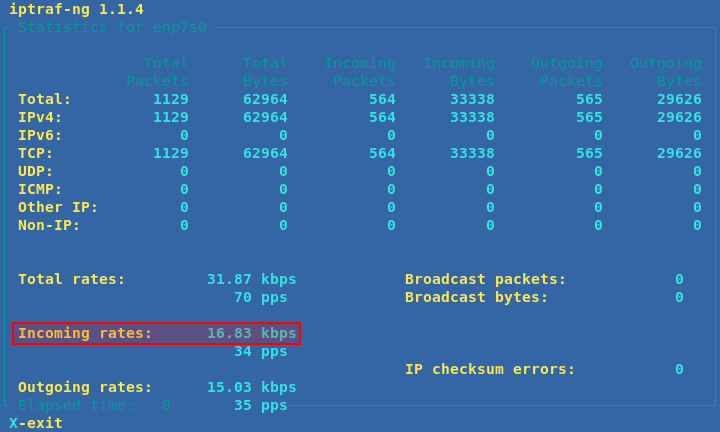
\includegraphics[width=1\textwidth]{figuras/consumo_banda_unfiltered.png}
	\caption{Consumo dos recursos de rede durante o recebimento de coordenadas sem filtragem.}
	\label{fig:consumo_banda_coord_unfiltered}
\end{figure}

\begin{figure}[H]
	\centering
	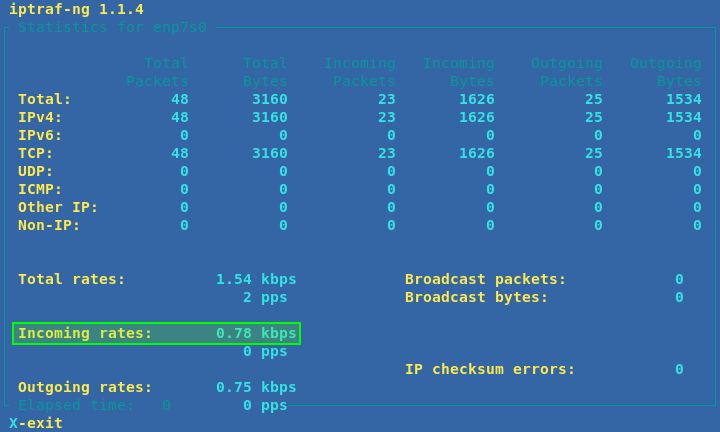
\includegraphics[width=1\textwidth]{figuras/consumo_banda_filtered.png}
	\caption{Consumo dos recursos de rede durante o recebimento de coordenadas com filtragem.}
	\label{fig:consumo_banda_coord_filtered}
\end{figure}

A banda de dados consumida pelo envio de coordenadas, foi minimizada pela aplicação de um filtro, que compara a última coordenada válida com a que será enviada, conforme explicado no final da \autoref{subsec:assemmodcapmov}. Desse modo, somente as modificações de posição são enviadas ao MCM. O resultado da aplicação desse filtro pode ser visualizado comparando-se a \autoref{fig:consumo_banda_coord_unfiltered} e a \autoref{fig:consumo_banda_coord_filtered}. Os testes de rede rodaram por aproximadamente 10 segundos com o MCM acoplado à cabeça do operador em posição de repouso (movimento mínimo).\par

A \autoref{fig:consumo_banda_vídeo} mostra o consumo de banda de dados quando o MCC está transmitindo o vídeo capturado pela câmera. Vale notar que a soma de recursos de rede, consumidos pelas funções de envio de coordenada e de transmissão de vídeo, não ultrapassam a banda disponível de 100Mbps. Portanto, afasta-se a possibilidade de esgotamento de banda de dados, que impediria a comunicação correta entre os módulos.\par

\begin{figure}[H]
	\centering
	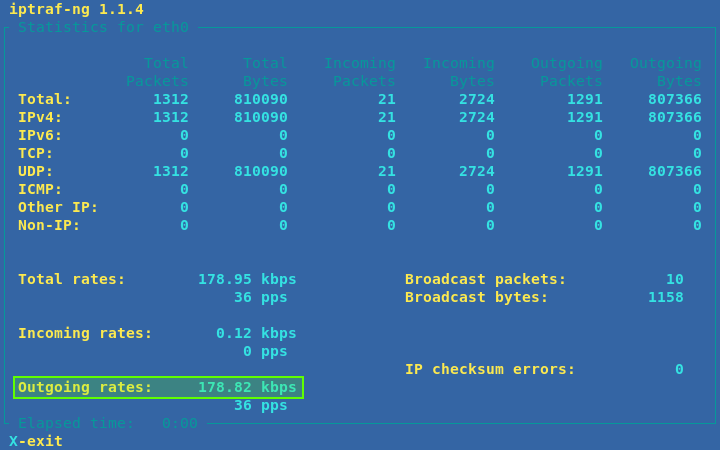
\includegraphics[width=1\textwidth]{figuras/consumo_banda_camera.png}
	\caption{Consumo dos recursos de rede durante o envio de imagem da câmera.}
	\label{fig:consumo_banda_vídeo}
\end{figure}

\subsection{Comparação Entre \textit{Codecs}}
\label{subsec:compcodecs}

Dentre os testes realizados com alguns dos \textit{codecs} de vídeo, compatíveis com o FFmpeg, os que mais chamaram atenção e que representaram um ganho considerável, em relação ao custo computacional, foram os \textit{codecs} \textbf{h264\_omx} e \textbf{h264}, implementados em \textit{hardware} e \textit{software} respectivamente.
Comparando-se a \autoref{fig:top_ffmpeg_h264_omx} e a \autoref{fig:top_ffmpeg_h264}, obtidas da interface do gerenciador de tarefas \textit{top}, fica claro que a implementação de \textit{codecs} via \textit{hardware} traz um ganho considerável em tempo de processador e quantidade de memória \textit{RAM} alocada. Existe um ganho de aproximadamente 28\% em tempo de processador e 35\% em uso de memória \textit{RAM}. Uma parte do uso de recursos nas duas figuras está relacionada ao processo de \textit{streaming}, implementada via \textit{software}. Como o \textit{streaming} é o mesmo para as duas comparações, não existe inconsistência na comparação.

\begin{figure}[H]
	\centering
	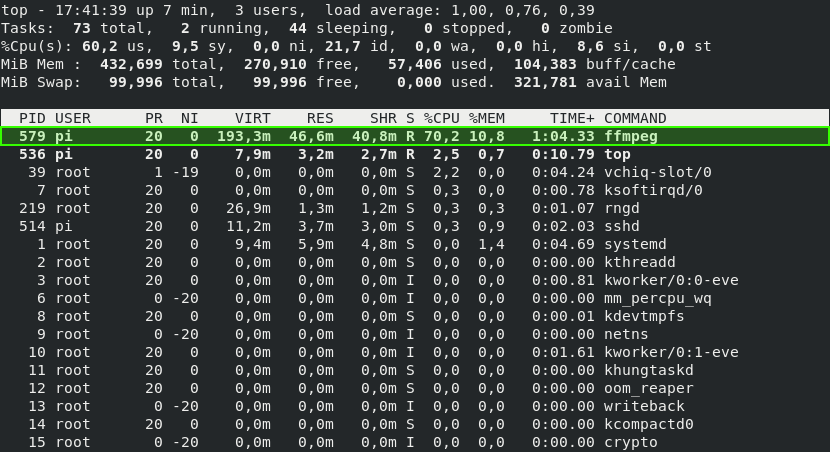
\includegraphics[width=1\textwidth]{figuras/top_ffmpeg_h264_omx.png}
	\caption{Consumo de recursos de \textit{hardware} pelo FFmpeg usando o codec h264\_omx, implementado em \textit{hardware}.}
	\label{fig:top_ffmpeg_h264_omx}
\end{figure}

\begin{figure}[H]
	\centering
	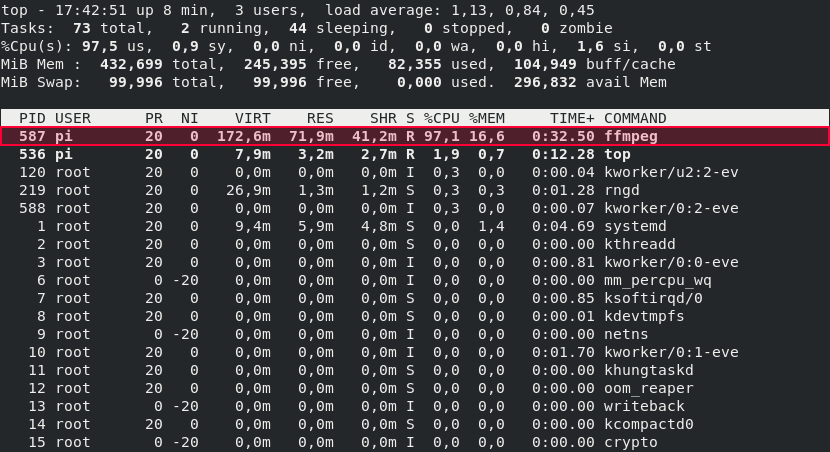
\includegraphics[width=1\textwidth]{figuras/top_ffmpeg_h264.png}
	\caption{Consumo de recursos de \textit{hardware} pelo FFmpeg usando o codec h264, implementado em \textit{software}.}
	\label{fig:top_ffmpeg_h264}
\end{figure}

	%% ORIENTAÇÕES GERAIS------------------------------------------------------------


% SOBRE AS ILUSTRAÇÕES----------------------------------------------------------
\chapter{SOBRE AS ILUSTRAÇÕES}
\label{chap:apSobreIlust}

A seguir exemplifica-se como inserir ilustrações no corpo do trabalho. As ilustrações serão indexadas automaticamente em suas respectivas listas. A numeração sequencial de figuras, tabelas e equações também ocorre de modo automático.

Referências cruzadas são obtidas através dos comandos \verb|\label{}| e \verb|\ref{}|. Sendo assim, não é necessário por exemplo, saber que o número de certo capítulo é \ref{chap:fundamentacaoTeorica} para colocar o seu número no texto. Outra forma que pode ser utilizada é esta: \autoref{chap:fundamentacaoTeorica}, facilitando a inserção, remoção e manejo de elementos numerados no texto sem a necessidade de renumerar todos esses elementos.

% FIGURAS-----------------------------------------------------------------------
\chapter{FIGURAS}
\label{chap:figuras}

Exemplo de como inserir uma figura. A \autoref{fig:figura-exemplo1} aparece automaticamente na lista de figuras. Para saber mais sobre o uso de imagens no \LaTeX{} consulte literatura especializada \cite{Goossens2007}.

Os arquivos das figuras devem ser armazenados no diretório de "/dados".

\begin{figure}[!htb]
    \centering
    \caption{Exemplo de Figura}
    \includegraphics[width=0.5\textwidth]{./dados/figuras/figura1}
    \fonte{\citeonline{IRL2014}}
    \label{fig:figura-exemplo1}
\end{figure}

% QUADROS E TABELAS---------------------------------------------------------------
\chapter{QUADROS E TABELAS}
\label{chap:tabelas}

Exemplo de como inserir o \autoref{qua:quadro-exemplo1} e a \autoref{tab:tabela-exemplo1}. Ambos aparecem automaticamente nas suas respectivas listas. Para saber mais informações sobre a construção de tabelas no \LaTeX{} consulte literatura especializada \cite{Mittelbach2004}.

Ambos os elementos (Quadros e Tabelas) devem ser criados em arquivos separados para facilitar manutenção e armazenados no diretório de "/dados".

\input{./dados/quadros/quadro1}

A diferença entre quadro e tabela está no fato que um quadro é formado por linhas horizontais e verticais. Deve ser utilizado quando o conteúdo é majoritariamente não-numérico. O número do quadro e o título vem acima do quadro, e a fonte, deve vir abaixo. E Uma tabela é formada apenas por linhas verticais. Deve ser utilizada quando o conteúdo é majoritariamente numérico. O número da tabela e o título vem acima da tabela, e a fonte, deve vir abaixo, tal como no quadro.

\begin{table}[!htb]
    \centering
    \caption[Resultado dos testes]{Resultado dos testes.
    \label{tab:tabela-exemplo1}}
    \begin{tabular}{rrrrr}
        \toprule
            & Valores 1 & Valores 2 & Valores 3 & Valores 4 \\
        \midrule
            Caso 1 & 0,86 & 0,77 & 0,81 & 163 \\
            Caso 2 & 0,19 & 0,74 & 0,25 & 180 \\
            Caso 3 & 1,00 & 1,00 & 1,00 & 170 \\
        \bottomrule
    \end{tabular}
    \fonte{XXXXXXXX}
\end{table}


% EQUAÇÕES-----------------------------------------------------------------------
\chapter{EQUAÇÕES}
\label{chap:equacoes}

Exemplo de como inserir a \autoref{eq:equacao-exemplo1} e a Eq. \ref{eq:equacao-exemplo2} no corpo do texto \footnote{Deve-se atentar ao fato de a formatação das equações ficar muito boa esteticamente.}. Observe que foram utilizadas duas formas distintas para referenciar as equações.

\begin{equation}
    X(s) = \int\limits_{t = -\infty}^{\infty} x(t) \, \text{e}^{-st} \, dt
    \label{eq:equacao-exemplo1}
\end{equation}

\begin{equation}
    F(u, v) = \sum_{m = 0}^{M - 1} \sum_{n = 0}^{N - 1} f(m, n) \exp \left[ -j 2 \pi \left( \frac{u m}{M} + \frac{v n}{N} \right) \right]
    \label{eq:equacao-exemplo2}
\end{equation}

% ALGORITMOS-----------------------------------------------------------------------
\chapter{ALGORITMOS}
\label{chap:algoritmos}

Exemplo de como inserir um algoritmo. Para inserção de algoritmos utiliza-se o pacote {\ttfamily algorithm2e} que já está devidamente configurado dentro do template.

Os algoritmos devem ser criados em arquivos separados para facilitar manutenção e armazenados no diretório de "/dados".\\
\\

\input{./dados/algoritmos/algoritmo1}

% SOBRE AS LISTAS--------------------------------------------------------------------
\chapter{SOBRE AS LISTAS}
\label{chap:apSobreLista}

Para construir listas de "\textit{bullets}"{} ou listas enumeradas, inclusive listas aninhadas, é utilizado o pacote \verb|paralist|.

Exemplo de duas listas não numeradas aninhadas, utilizando o comando \verb|\itemize|. Observe a indentação, bem como a mudança automática do tipo de "\textit{bullet}"{} nas listas aninhadas.

\begin{itemize}
    \item item não numerado 1
    \item item não numerado 2
    \begin{itemize}
        \item subitem não numerado 1
        \item subitem não numerado 2
        \item subitem não numerado 3
    \end{itemize}
    \item item não numerado 3
\end{itemize}

Exemplo de duas listas numeradas aninhadas, utilizando o comando \verb|\enumerate|. Observe a numeração progressiva e indentação das listas aninhadas.

\begin{enumerate}
    \item item numerado 1
    \item item numerado 2
    \begin{enumerate}
        \item subitem numerado 1
        \item subitem numerado 2
        \item subitem numerado 3
    \end{enumerate}
    \item item numerado 3
\end{enumerate}

% SOBRE AS CITAÇÕES E CHAMADAS DE REFERÊNCAS----------------------------------------------
\chapter{SOBRE AS CITAÇÕES E CHAMADAS DE REFERÊNCAS}
\label{chap:apSobreCita}

Citações são trechos de texto ou informações obtidas de materiais consultadss quando da elaboração do trabalho. São utilizadas no texto com o propósito de esclarecer, completar e embasar as ideias do autor. Todas as publicações consultadas e utilizadas (por meio de citações) devem ser listadas, obrigatoriamente, nas referências bibliográficas, para preservar os direitos autorais. São classificadas em citações indiretas e diretas.

% CITAÇÕES INDIRETAS-----------------------------------------------------------------------
\chapter{CITAÇÕES INDIRETAS}
\label{chap:citacoesLivres}

É a transcrição, com suas próprias palavras, das idéias de um autor, mantendo-se o sentido original. A citação indireta é a maneira que o pesquisador tem de ler, compreender e gerar conhecimento a partir do conhecimento de outros autores. Quanto à chamada da referência, ela pode ser feita de duas maneiras distintas, conforme o nome do(s) autor(es) façam parte do seu texto ou não. Exemplo de chamada fazendo parte do texto:\\
\\Enquanto \citeonline{Maturana2003} defendem uma epistemologia baseada na biologia. Para os autores, é necessário rever \ldots.\\

A chamada de referência foi feita com o comando \verb|\citeonline{chave}|, que produzirá a formatação correta.

A segunda forma de fazer uma chamada de referência deve ser utilizada quando se quer evitar uma interrupção na sequência do texto, o que poderia, eventualmente, prejudicar a leitura. Assim, a citação é feita e imediatamente após a obra referenciada deve ser colocada entre parênteses. Porém, neste caso específico, o nome do autor deve vir em caixa alta, seguido do ano da publicação. Exemplo de chamada não fazendo parte do texto:\\
\\Há defensores da epistemologia baseada na biologia que argumentam em favor da necessidade de \ldots \cite{Maturana2003}.\\

Nesse caso a chamada de referência deve ser feita com o comando \verb|\cite{chave}|, que produzirá a formatação correta.

% CITAÇÕES DIRETAS-----------------------------------------------------------------------
\chapter{CITAÇÕES DIRETAS}
\label{chap:citacoesLiterais}

É a transcrição ou cópia de um parágrafo, de uma frase, de parte dela ou de uma expressão, usando exatamente as mesmas palavras adotadas pelo autor do trabalho consultado.

Quanto à chamada da referência, ela pode ser feita de qualquer das duas maneiras já mencionadas nas citações indiretas, conforme o nome do(s) autor(es) façam parte do texto ou não. Há duas maneiras distintas de se fazer uma citação direta, conforme o trecho citado seja longo ou curto.

Quando o trecho citado é longo (4 ou mais linhas) deve-se usar um parágrafo específico para a citação, na forma de um texto recuado (4 cm da margem esquerda), com tamanho de letra menor e espaçamento entrelinhas simples. Exemplo de citação longa:
\\\begin{citacao}
    Desse modo, opera-se uma ruptura decisiva entre a reflexividade filosófica, isto é a possibilidade do sujeito de pensar e de refletir, e a objetividade científica. Encontramo-nos num ponto em que o conhecimento científico está sem consciência. Sem consciência moral, sem consciência reflexiva e também subjetiva. Cada vez mais o desenvolvimento extraordinário do conhecimento científico vai tornar menos praticável a própria possibilidade de reflexão do sujeito sobre a sua pesquisa \cite[p.~28]{Silva2000}.
\end{citacao}

Para fazer a citação longa deve-se utilizar os seguintes comandos:
\begin{verbatim}
\begin{citacao}
<texto da citacao>
\end{citacao}
\end{verbatim}

No exemplo acima, para a chamada da referência o comando \verb|\cite[p.~28]{Silva2000}| foi utilizado, visto que os nomes dos autores não são parte do trecho citado. É necessário também indicar o número da página da obra citada que contém o trecho citado.

Quando o trecho citado é curto (3 ou menos linhas) ele deve inserido diretamente no texto entre aspas. Exemplos de citação curta:\\
\\A epistemologia baseada na biologia parte do princípio de que "assumo que não posso fazer referência a entidades independentes de mim para construir meu explicar" \cite[p.~35]{Maturana2003}.\\
\\A epistemologia baseada na biologia de \citeonline[p.~35]{Maturana2003} parte do princípio de que "assumo que não posso fazer referência a entidades independentes de mim para construir meu explicar".

% DETALHES SOBRE AS CHAMADAS DE REFERÊNCIAS---------------------------------------------------------
\chapter{DETALHES SOBRE AS CHAMADAS DE REFERÊNCIAS}
\label{chap:referUtilizadas}

Outros exemplos de comandos para as chamadas de referências e o resultado produzido por estes:\\
\\\citeonline{Maturana2003} \ \ \  \verb|\citeonline{Maturana2003}|\\
\citeonline{Barbosa2004} \ \ \   \verb|\citeonline{Barbosa2004}|\\
\cite[p.~28]{Silva2000} \ \ \  \verb|\cite[p.~28]{Silva2000}|\\
\citeonline[p.~33]{Silva2000} \ \ \   \verb|\citeonline[p.~33]{v}|\\
\cite[p.~35]{Maturana2003} \ \ \   \verb|\cite[p.~35]{Maturana2003}|\\
\citeonline[p.~35]{Maturana2003} \ \ \   \verb|\citeonline[p.~35]{Maturana2003}|\\
\cite{Barbosa2004,Maturana2003} \ \ \   \verb|\cite{Barbosa2004,Maturana2003}|\\

% SOBRE AS REFERÊNCIAS BIBLIOGRÁFICAS-------------------------------------------------------
\chapter{SOBRE AS REFERÊNCIAS BIBLIOGRÁFICAS}
\label{chap:apSobreRefer}

A bibliografia é feita no padrão \textsc{Bib}\TeX{}. As referências são colocadas em um arquivo separado. Neste template as referências são armazenadas no arquivo "base-referencias.bib".

Existem diversas categorias documentos e materiais componentes da bibliografia. A classe abn\TeX{} define as seguintes categorias (entradas):

\begin{verbatim}
@book
@inbook
@article
@phdthesis
@mastersthesis
@monography
@techreport
@manual
@proceedings
@inproceedings
@journalpart
@booklet
@patent
@unpublished
@misc
\end{verbatim}

Cada categoria (entrada) é formatada pelo pacote \citeonline{abnTeX22014d} de uma forma específica. Algumas entradas foram introduzidas especificamente para atender à norma \citeonline{NBR6023:2002}, são elas: \verb|@monography|, \verb|@journalpart|,\verb|@patent|. As demais entradas são padrão \textsc{Bib}\TeX{}. Para maiores detalhes, refira-se a \citeonline{abnTeX22014d}, \citeonline{abnTeX22014b}, \citeonline{abnTeX22014c}.

% NOTAS DE RODAPÉ--------------------------------------------------------------------------
\chapter{NOTAS DE RODAPÉ}
\label{chap:notasRodape}

As notas de rodapé pode ser classificadas em duas categorias: notas explicativas\footnote{é o tipo mais comum de notas que destacam, explicam e/ou complementam o que foi dito no corpo do texto, como esta nota de rodapé, por exemplo.} e notas de referências. A notas de referências, como o próprio nome ja indica, são utilizadas para colocar referências e/ou chamadas de referências sob certas condições.

                  % Capítulo com Orientações de uso do Template, depois pode-se ocultar com o símbolo de porcentagem
	% CONCLUSÃO--------------------------------------------------------------------

\chapter{CONCLUSÃO}
\label{chap:conclusao}

Este trabalho apresenta o desenvolvimento de um sistema do tipo \textit{Pan} e \textit{Tilt}, para controle remoto de câmera, com base no movimento da cabeça do operador, capturado por sensores de um celular, acoplado ao usuário através de um óculos do tipo \textit{VR}.\par
Com base nos resultados obtidos, e corrigindo-se questões pertinentes ao envio de imagens de video, um sistema semelhante ao construído, pode ser utilizado para facilitar o manuseio, ou operação, de um dispositivo de inspeção. Sendo assim, um operador pode usar os movimentos de sua cabeça para controlar a câmera de um robô, reduzindo o numero de ações vinculada ao controle manual, normalmente necessárias para movimentar o robô, suas ferramentas e a câmera embarcada. \par 
O sistema de imagem \textit{stereo}, aumenta a percepção do local, uma vez que adiciona a sensação de profundidade às imagens, facilita a locomoção, a orientação e, consequentemente, a inspeção de ambientes.

O projeto foi elaborado usando um \textit{Raspberry Pi}, como unidade computacional e de controle dos servo motores da câmera, e um celular \textit{smartphone} \textit{Android}, responsável por coletar e enviar informações referentes a posição espacial do aparelho. O desenvolvimento do projeto proporcionou um melhor entendimento em aspetos relacionados a rede de computadores, sistemas operacionais, interfaces de hardware, modulação por largura de pulso, eletrônica e desenvolvimento de sistemas para plataformas móveis.\par

Competências ligadas a construção de software puderam ser evoluídas, já que o módulo de controle, embarcado no Raspberry Pi, foi construído em linguagem C e o módulo de coleta de dados foi desenvolvido em Java, usando a API do sistema operacional Android.\par

\section{Trabalhos Futuros}
\label{sec:trabalhosFuturos}

\begin{itemize}
\item Corrigir problemas relacionados ao envio de imagens video para o celular.
\item Desenvolver um mecanismo automático de calibração do celular (independente da orientação magnética do planeta)
\item Criar um modo de tela cheia para melhor visualização das imagens com o óculos de realidade virtual.
\item Adicionar suporte a conexão \textit{bluetooth} entre um \textit{joysticks} e o celular, permitindo interação com a interface de teste e enviar comandos para o robô.
\item Criar uma API para possibilitar a integração com outras soluções (ex: mostrar dados capturados de sensores embarcados na imagem enviada para o celular).
\item Adicionar captura de som \textit{stereo} no módulo de controle dos motores.
\item Transmitir o sinal de som capturado junto com o vídeo para o celular, aumentando a sensação de imersão para o operador.
\item Melhoria do sistema de alimentação para a solução (tornar portátil).
\item Construir uma placa para evitar o mau contato entre componentes eletrônicos no circuito de acionamento dos motores (construção de uma \textit{Raspberry Pi hat}).
\end{itemize}
                 			           % Conclusão
	

	\postextual
	% INSERE ELEMENTOS PÓS-TEXTUAIS
	% REFERÊNCIAS------------------------------------------------------------------

% Carrega o arquivo "base-referencias.bib" e extrai automaticamente as referências citadas

\bibliography{./base-referencias}
\bibliographystyle{abntex2-alf} % Define o estilo ABNT para formatar a lista de referências
% OBSERVAÇÕES------------------------------------------------------------------
% Este arquivo não precisa ser alterado.
           			   % Referências
	% APÊNDICES--------------------------------------------------------------------

\begin{apendicesenv}
\partapendices



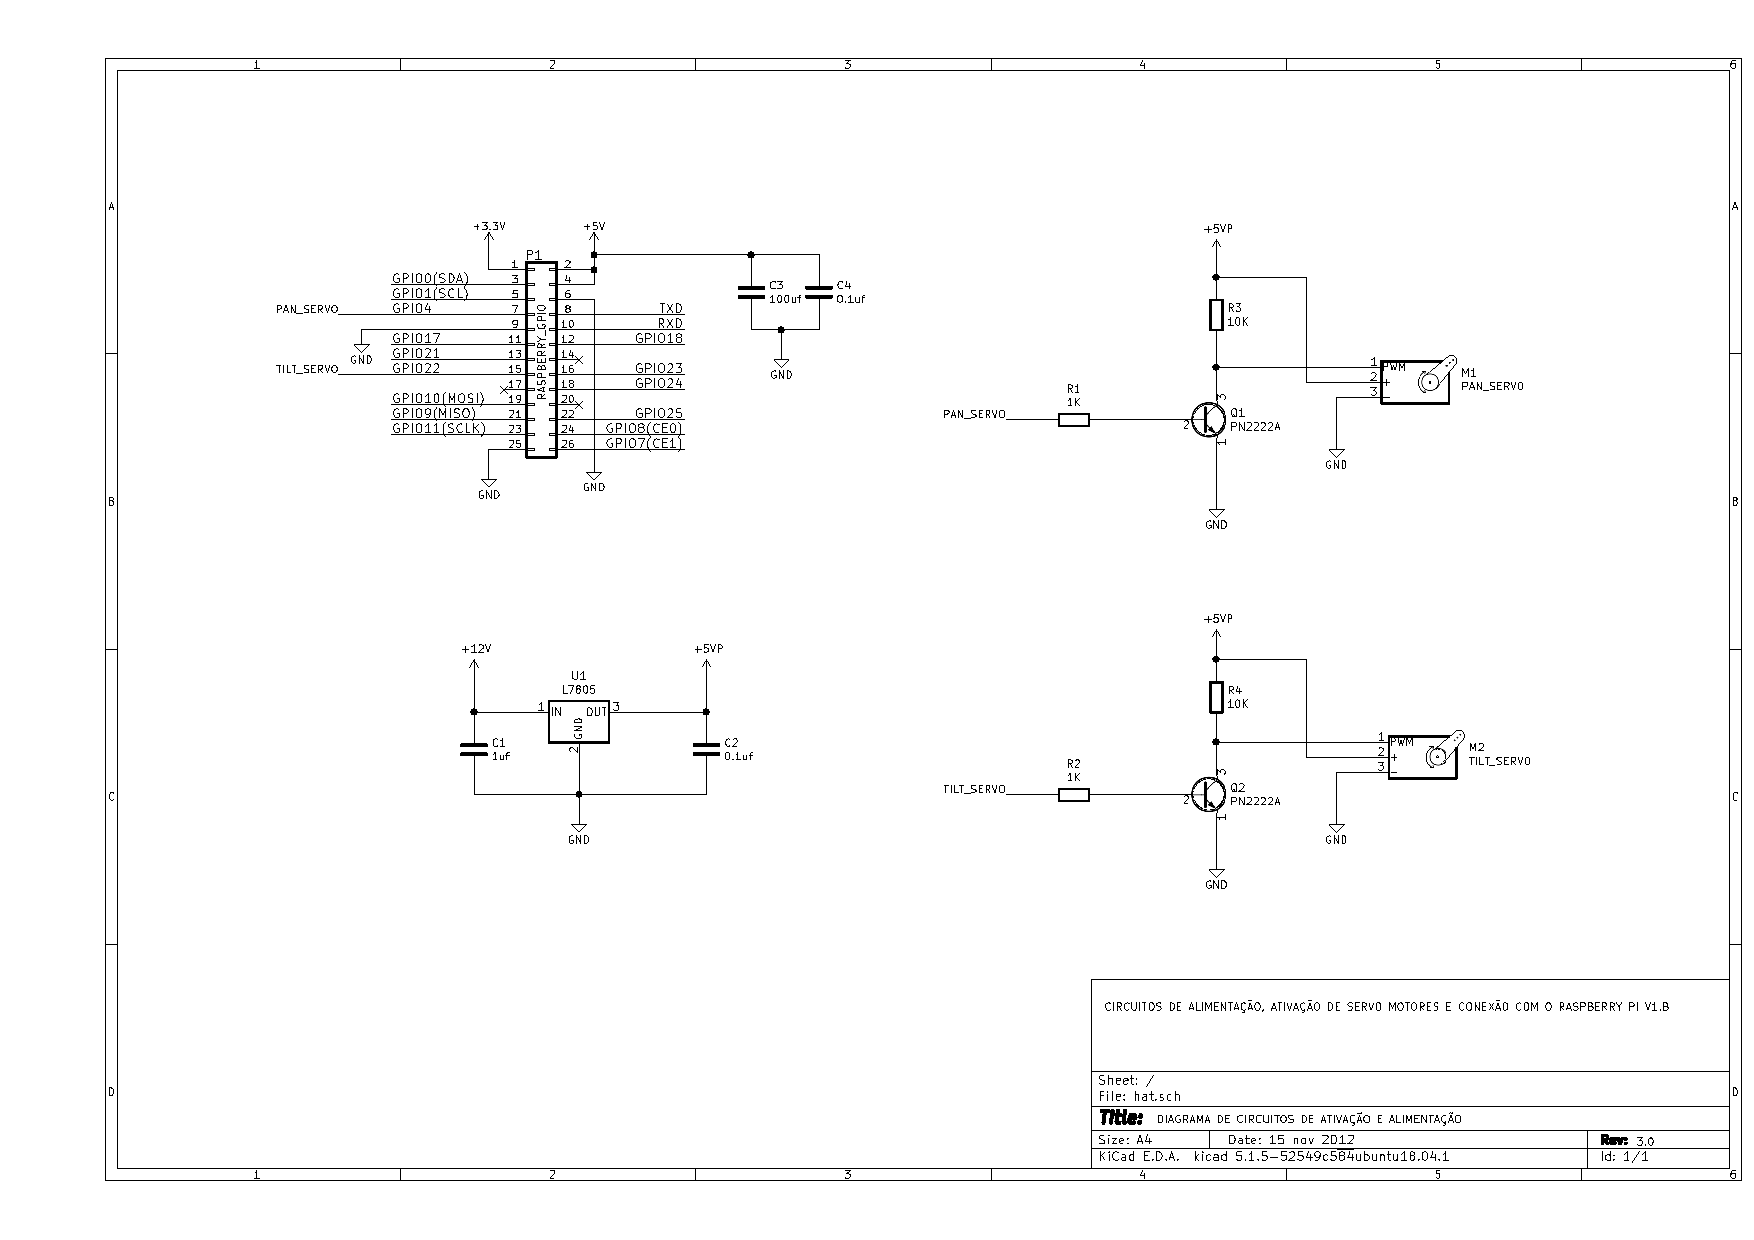
\includepdf[pages=-,offset=0 -20,angle=-90,scale=0.9,pagecommand={
	\chapter{Diagrama de Circuitos} % Edite para alterar o título deste apêndice
	\label{chap:board}
}]{../board/hat.pdf}

\chapter{Fotos do Protótipo} % Edite para alterar o título deste apêndice
\label{chap:fotosprototipo}

\begin{figure}[H]
	\centering
	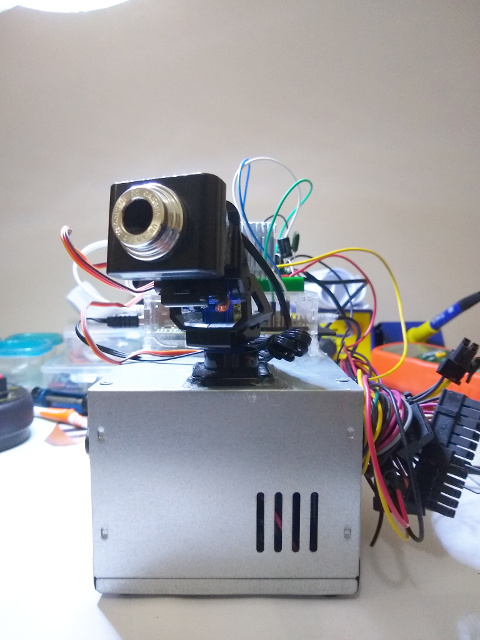
\includegraphics[width=1\linewidth]{figuras/vista_frontal}
	\caption{Visão frontal.}
	\label{fig:vistafrontal}
\end{figure}

\begin{figure}[H]
	\centering
	\includegraphics[width=1\linewidth]{figuras/vista_traseira}
	\caption{Visão traseira.}
	\label{fig:vistatraseira}
\end{figure}

\begin{figure}[H]
	\centering
	\includegraphics[width=1\linewidth]{figuras/vista_esquerda}
	\caption{Visão lateral esquerda.}
	\label{fig:vistaesquerda}
\end{figure}

\begin{figure}[H]
	\centering
	\includegraphics[width=1\linewidth]{figuras/vista_direita}
	\caption{Visão lateral direita.}
	\label{fig:vistadireita}
\end{figure}

\begin{figure}[H]
	\centering
	\includegraphics[width=1\linewidth]{figuras/vista_superior}
	\caption{Visão superior.}
	\label{fig:vistasuperior}
\end{figure}

\begin{figure}[H]
	\centering
	\includegraphics[width=1\linewidth]{figuras/vista_detalhe_fixacao_camera}
	\caption{Fixação da câmera com cola quente.}
	\label{fig:vistadetalhefixacaocamera}
\end{figure}

\begin{figure}[H]
	\centering
	\includegraphics[width=1\linewidth]{figuras/vista_detalhe_fixacao_raspi}
	\caption{Fixação do gabinete do \textit{Raspberry Pi} com cola quente.}
	\label{fig:vistadetalhefixacaoraspi}
\end{figure}

\begin{figure}[H]
	\centering
	\includegraphics[width=1\linewidth]{figuras/vista_detalhe_circuito}
	\caption{Detalhe da montagem do circuito na mini \textit{breadboard}.}
	\label{fig:vistadetalhecircuito}
\end{figure}

\end{apendicesenv}
             		   % Apêndices
	% ANEXO------------------------------------------------------------------------

\begin{anexosenv}
\partanexos

% Primeiro anexo---------------------------------------------------------------
\chapter{Nome do anexo}     % edite para alterar o título deste anexo
\label{chap:anexoA}

Lembre-se que a diferença entre apêndice e anexo diz respeito à autoria do texto e/ou material ali colocado.

Caso o material ou texto suplementar ou complementar seja de sua autoria, então ele deverá ser colocado como um apêndice. Porém, caso a autoria seja de terceiros, então o material ou texto deverá ser colocado como anexo.

Caso seja conveniente, podem ser criados outros anexos para o seu trabalho acadêmico. Basta recortar e colar este trecho neste mesmo documento. Lembre-se de alterar o "label"{} do anexo.

Organize seus anexos de modo a que, em cada um deles, haja um único tipo de conteúdo. Isso facilita a leitura e compreensão para o leitor do trabalho. É para ele que você escreve.

% Novo anexo-------------------------------------------------------------------
\chapter{Nome do outro anexo}
\label{chap:anexoB}

conteúdo do outro anexo

\end{anexosenv}
               			   % Anexos
	\end{OnehalfSpace}

\end{document}
